\documentclass[@BEAMER_OPTIONS@]{beamer}
    @USE_PGFPAGES@

    \usetheme[alternativetitlepage=true,titleline=true]{Torino}
    \setbeamertemplate{navigation symbols}{}
    \setbeamertemplate{note page}[plain]
    \setbeamertemplate{caption}{\insertcaption}

    \usepackage[utf8]{inputenc}
    \usepackage[russian]{babel}
    \usepackage{graphicx}
    \usepackage{subfigure}
    \usepackage{xspace}
    \usepackage{adjustbox}
    \usepackage{tikz}
    \usepackage{relsize}
    \usepackage{fancyvrb}
    \fvset{fontsize=\footnotesize}
    \RecustomVerbatimEnvironment{verbatim}{Verbatim}{}
    \usepgflibrary{arrows}
    \usetikzlibrary{shadows,decorations.pathreplacing,patterns,shapes}
    \tikzstyle{every picture}=[semithick,>=stealth,remember picture]
    \usepackage{inconsolata}
    \usepackage{listings}
    \lstset{
        language=C++,
        basicstyle=\footnotesize\rmfamily,
        keywordstyle=\color{chameleon1}\bfseries,
        commentstyle=\color{chameleon4}\it\rmfamily,
        stringstyle=\color{chameleon4},
        numbers=left,
        numberstyle=\tiny,
        aboveskip=-0.02\baselineskip,
        belowskip=-0.02\baselineskip,
        columns=flexible,
        extendedchars=false,
        showstringspaces=false,
        morekeywords={global,kernel,ulong,size_t,cl_uint,cl_platform_id}
        }
    \newcommand{\code}[1]{\lstinline|#1|}
    \protected\def\plusplus{{\nolinebreak[4]\hspace{-.05em}\raisebox{.4ex}{\relsize{-3}\bf ++}}\xspace}
    \newcommand{\CXX}{{\rm C}\plusplus}
    \newcommand{\CC}{{\rm C99}\xspace}
    \newcommand{\www}[1]{\href{#1}{#1}}

    \usepackage{ifthen}
\usetikzlibrary{shadows.blur}
\newlength{\ribbonoffset}
\setlength{\ribbonoffset}{3em}

% corner, color, text
\newcommand{\ribbon}[3]{
  \ifthenelse{\equal{#1}{east}}{%
    \tikzset{ribbonrot/.style={rotate=-45}}
  }{%
    \tikzset{ribbonrot/.style={rotate=45}}
  }
  \begin{tikzpicture}[remember picture, overlay]
    \node[ribbonrot, shift={(0, -\ribbonoffset)}] at (current page.north #1) {
      \begin{tikzpicture}[remember picture, overlay,scale=0.5]
        \node[
            fill=#2,
            text centered,
            minimum width=50em,
            minimum height=1.2em,
            blur shadow,
            shadow yshift=0pt,
            shadow xshift=0pt,
            shadow blur radius=.2em,
            shadow opacity=50,
            text=white
            ](fmogh) at (0pt, 0pt) {%
            \fontfamily{phv}\selectfont\bfseries\tiny#3};
        \draw[
            white,
            dashed,
            line width=.04em,
            dash pattern=on .2em off 1.5\pgflinewidth
            ] (-25em,1em) rectangle (25em,-1em);
      \end{tikzpicture}
    };
  \end{tikzpicture}
}

    \newcommand{\forkme}{\ribbon{east}{chameleon1}{\href{https://github.com/ddemidov/vexcl}{Fork me on GitHub}}}
    \newcommand{\singledevice}{\ribbon{east}{chameleon3}{1xGPU}}
    \newcommand{\additive}{\ribbon{east}{chameleon3}{Additive expressions}}
    \newcommand{\speakerdeck}{%
        \begin{tikzpicture}[remember picture, overlay]%
            \node[%
                shift={(45pt,10pt)},
                text centered,%
                text=black%
                ] at (current page.south west)%
            {\tiny\href{https://speakerdeck.com/ddemidov}{speakerdeck.com/ddemidov}};%
        \end{tikzpicture}%
    }

    \tikzset{
        treenode/.style={
            draw,
            fill=white,
            blur shadow,
            shadow xshift=1pt,
            shadow yshift=-1pt,
            shadow blur radius=2pt,
            shadow opacity=40
            }
        }


    \title{Программирование OpenCL}
    \subtitle{с использованием библиотек \CXX}
    \author{Денис Демидов}
    \institute{Институт системных исследований РАН\\
    Казанский Федеральный Университет}
    \date{23.10.2015}


\begin{document}

%----------------------------------------------------------------------------
\begin{frame}{}
    \titlepage
    \speakerdeck
\end{frame}

\note{ }

%----------------------------------------------------------------------------
\section{Введение}

\begin{frame}{Современные GPGPU платформы}
    \begin{columns}
        \begin{column}{0.45\textwidth}
            \begin{block}{CUDA}
                \begin{itemize}
                    \item Проприетарная архитектура
                    \item Работает только на видеокартах NVIDIA
                    \item Высокоуровневый интерфейс
                    \item Ядра (\CXX) компилируются в псевдокод (PTX) вместе с
                        основной программой
                \end{itemize}
            \end{block}
        \end{column}
        \begin{column}{0.45\textwidth}
            \begin{block}{OpenCL}
                \begin{itemize}
                    \item Открытый стандарт
                    \item Поддерживается многими вендорами
                    \item Низкоуровневый интерфейс
                    \item Ядра (\CC) компилируются во время выполнения основной
                        программы
                \end{itemize}
            \end{block}
        \end{column}
    \end{columns}
\end{frame}

\note[itemize]{
\item Today, major GPGPU programming frameworks are NVIDIA CUDA and OpenCL
\item ...
\item The latter distinction allows one to generate an OpenCL kernel tailored
    for the problem at hand.  And that is what I am going to talk about today.
}

\begin{frame}{Поддерживаемые устройства}
    \begin{itemize}
        \item NVIDIA CUDA
            \begin{itemize}
                \item Видеокарты NVIDIA
            \end{itemize}
        \item OpenCL
            \begin{itemize}
                \item Видеокарты NVIDIA, AMD, Intel
                \item Центральные процессоры Intel, AMD, ARM
                \item Мобильные системы, программируемые чипы, \ldots
            \end{itemize}
    \end{itemize}
\end{frame}

\section{Программный интерфейс OpenCL}
\begin{frame}
    \sectionpage
\end{frame}

\begin{frame}{Справочная информация}
    \begin{itemize}
        \item Сайт группы компаний Khronos
            \begin{itemize}
                \item Спецификации: \href{http://khronos.org/registry/cl}{khronos.org/registry/cl}
                \item Ресурсы: \href{http://khronos.org/opencl/resources}{khronos.org/opencl/resources}
            \end{itemize}
    \end{itemize}
\end{frame}

\begin{frame}{Основные этапы при использовании OpenCL}
    \begin{itemize}
        \item Инициализация
            \begin{itemize}
                \item Выбор платформы
                \item Выбор устройства
                \item Создание контекста
                \item Создание очереди команд
                \item Выделение памяти на устройстве
                \item Компиляция вычислительных ядер
            \end{itemize}
        \item Работа
            \begin{itemize}
                \item Перенос данных
                \item Выполнение расчетов
            \end{itemize}
    \end{itemize}
\end{frame}

\begin{frame}[fragile]{Платформа OpenCL}
    \begin{description}
        \item[Платформа] --- это конкретная реализация OpenCL от производителя
            аппаратного обеспечения (AMD, Intel, Nvidia, и т.д.)
    \end{description}

    Платформа позволяет получить:
    \begin{itemize}
        \item Свойства платформы:
            \begin{itemize}
                \item \code{CL_PLATFORM_NAME}
                \item \code{CL_PLATFORM_VERSION}
                \item \code{CL_PLATFORM_VENDOR}
            \end{itemize}
        \item Список установленных устройств, поддерживаемых платформой
    \end{itemize}
\end{frame}

\begin{frame}[fragile]{С интерфейс}
    \begin{exampleblock}{}
        \begin{lstlisting}
#include <iostream>
#include <vector>
#include <stdexcept>
#include <CL/cl.h>

void check(cl_int return_code) {
    if (return_code != CL_SUCCESS) throw std::runtime_error("OpenCL error");
}
int main() {
    cl_uint np;
    check( clGetPlatformIDs(0, NULL, &np) );
    std::vector<cl_platform_id> platforms(np);
    check( clGetPlatformIDs(np, platforms.data(), &np) );
    char name[256];
    for (auto p : platforms) {
        check( clGetPlatformInfo(p, CL_PLATFORM_NAME, 256, name, NULL) );
        std::cout << name << std::endl;
    }
}
        \end{lstlisting}
    \end{exampleblock}
\end{frame}

\begin{frame}[fragile]{\CXX интерфейс}
    \begin{exampleblock}{}
        \begin{lstlisting}
#include <iostream>
#include <vector>

#define __CL_ENABLE_EXCEPTIONS
#include <CL/cl.hpp>

int main() {
    std::vector<cl::Platform> platforms;
    cl::Platform::get(&platforms);

    for (const auto &p : platforms)
        std::cout << p.getInfo<CL_PLATFORM_NAME>() << std::endl;
}
        \end{lstlisting}
    \end{exampleblock}
\end{frame}

\begin{frame}[fragile]{Устройство OpenCL}
    \begin{description}
        \item[Устройство] --- конкретное вычислительное устройство,
            поддерживаемое одной из установленных платформ.
    \end{description}
    \begin{exampleblock}{Получение списка устройств для платформы}
        \begin{lstlisting}
std::vector<cl::Device> devices;
p.getDevices(CL_DEVICE_TYPE_ALL, &devices);

for(const auto &d : devices)
    std::cout << "  " << d.getInfo<CL_DEVICE_NAME>() << std::endl;
        \end{lstlisting}
    \end{exampleblock}
    Типы устройств:
    \begin{itemize}
        \item \code{CL_DEVICE_TYPE_ALL}
        \item \code{CL_DEVICE_TYPE_DEFAULT}
        \item \code{CL_DEVICE_TYPE_CPU}
        \item \code{CL_DEVICE_TYPE_GPU}
        \item \code{CL_DEVICE_TYPE_ACCELERATOR}
    \end{itemize}
\end{frame}

\begin{frame}[fragile]{Контекст OpenCL}
    \begin{description}[\;\;]
        \item[Контекст] --- служит для управления объектами и ресурсами
            OpenCL.\\
            С контекстом связаны:
            \begin{itemize}
                \item устройства
                \item программы и ядра
                \item буферы памяти
                \item очереди команд
            \end{itemize}
    \end{description}
    \begin{exampleblock}{Создание контекста}
        \begin{lstlisting}
cl::Context context(devices);
        \end{lstlisting}
    \end{exampleblock}
\end{frame}

\begin{frame}[fragile]{Очередь команд}
    \begin{description}
        \item[Очередь команд] --- позволяет отправить задание на выполнение на
            конкретное устройство.
    \end{description}
    \begin{itemize}
        \item Очередь связана с единственными контекстом и устройством.
        \item Постановка задания в очередь выполняется асинхронно.
        \item Задания выполняются в порядке их постановки в очередь.
            \begin{itemize}
                \item Вычислительные ядра
                \item Операции копирования памяти
            \end{itemize}
    \end{itemize}
    \begin{exampleblock}{Создание очереди}
        \begin{lstlisting}
cl::CommandQueue queue(context, devices[0]);
        \end{lstlisting}
    \end{exampleblock}
\end{frame}

\begin{frame}[fragile]{Выделение и копирование памяти}
    \begin{description}[\;\;]
        \item[Буфер памяти] --- объект, владеющий некоторым объемом памяти в
            контексте.
            \begin{itemize}
                \item Все устройства в контексте могут получить доступ к
                    буферам памяти.
            \end{itemize}
    \end{description}
    \begin{exampleblock}{Выделение и перенос памяти}
        \begin{lstlisting}
std::vector<double> x(1024, 42.0);

cl::Buffer a(context, CL_MEM_READ_WRITE | CL_MEM_COPY_HOST_PTR,
        x.size() * sizeof(x[0]), x.data());

size_t nbytes = 1024 * sizeof(double);
cl::Buffer b(context, CL_MEM_READ_WRITE, nbytes);

queue.enqueueWriteBuffer(b, CL_FALSE, 0, nbytes, x.data());
queue.enqueueReadBuffer(b, CL_TRUE, 0, nbytes, x.data());
        \end{lstlisting}
    \end{exampleblock}
\end{frame}

\begin{frame}[fragile]{Создание вычислительного ядра}
    \begin{description}[\;\;]
        \item[Ядро] --- функция, исполняющаяся на вычислительном устройстве.
        \item[Программа] --- содержит исходные тесксты и/или скомпилированные
            ядра.
    \end{description}
    \begin{exampleblock}{Создание программы и ядра}
        \begin{lstlisting}
std::string source = R"(
kernel void add(ulong n, global const double *a, global double *b) {
    ulong i = get_global_id(0);
    if (i < n) b[i] += a[i];
}
)";

cl::Program program(context, source);
program.build(devices);

cl::Kernel add(program, "add");
        \end{lstlisting}
    \end{exampleblock}
\end{frame}

\begin{frame}[fragile]{Запуск ядра на выполнение}
    \begin{exampleblock}{Постановка ядра в очередь}
        \begin{lstlisting}
add.setArg(0, static_cast<cl_ulong>(n));
add.setArg(1, a);
add.setArg(2, b);

queue.enqueueNDRangeKernel(add, cl::NullRange, cl::NDRange(n), cl::NullRange);
        \end{lstlisting}
    \end{exampleblock}

    \begin{exampleblock}{Считывание результатов}
        \begin{lstlisting}
queue.enqueueReadBuffer(b, CL_TRUE, 0, nbytes, x.data());
std::cout << x[0] << std::endl;
        \end{lstlisting}
    \end{exampleblock}
\end{frame}

\section{Hello OpenCL}

\begin{frame}{Полный пример}
    \begin{itemize}
        \item Вычислить сумму двух векторов на видеокарте
            \begin{itemize}
                \item \code{A} и \code{B} --- векторы большой размерности
                \item Вычислить поэлементную сумму \code{B = A + B}.
            \end{itemize}
            \vspace{\baselineskip}
        \item Основные шаги
            \begin{enumerate}
                \item Инициализируем контекст
                \item Выделяем память
                \item Переносим входные данные
                \item Проводим вычисления
                \item Забираем результаты
            \end{enumerate}
    \end{itemize}
\end{frame}

\begin{frame}[fragile]{Hello OpenCL: Сумма двух векторов}
    \vspace{-1\baselineskip}
    \begin{columns}
        \begin{column}{0.2\textwidth}
            \begin{minipage}[c][\textheight][c]{\linewidth}
                \begin{exampleblock}{}
                    \begin{adjustbox}{width=0.19\textwidth, height=\textheight, keepaspectratio}
                        \begin{minipage}{\textwidth}
                            \begin{uncoverenv}<1->
                                \lstinputlisting[linerange={1-7}]{code/hello-opencl.cpp}
                            \end{uncoverenv}
                            \begin{uncoverenv}<2->
                                \lstinputlisting[firstnumber=last, linerange={8-33}]{code/hello-opencl.cpp}
                            \end{uncoverenv}
                            \begin{uncoverenv}<3->
                                \lstinputlisting[firstnumber=last, linerange={34-42}]{code/hello-opencl.cpp}
                            \end{uncoverenv}
                            \begin{uncoverenv}<4->
                                \lstinputlisting[firstnumber=last, linerange={43-68}]{code/hello-opencl.cpp}
                            \end{uncoverenv}
                            \begin{uncoverenv}<5->
                                \lstinputlisting[firstnumber=last, linerange={69-72}]{code/hello-opencl.cpp}
                            \end{uncoverenv}
                        \end{minipage}
                    \end{adjustbox}
                \end{exampleblock}
            \end{minipage}
        \end{column}
        \begin{column}{0.7\textwidth}
            \begin{minipage}[c][\textheight][c]{\linewidth}
                \begin{exampleblock}{\small%
                        \only<1>{Разрешаем выбрасывать исключения}%
                        \only<2>{Инициализируем контекст}%
                        \only<3>{Выделяем память}%
                        \only<4>{Компилируем и выполняем ядро}%
                        \only<5>{Забираем результаты}%
                    }
                    \begin{adjustbox}{width=0.7\textwidth, height=\textheight, keepaspectratio}
                        \begin{minipage}{\textwidth}
                            \begin{onlyenv}<1>
                                \lstinputlisting[linerange={1-7}]{code/hello-opencl.cpp}
                            \end{onlyenv}
                            \begin{onlyenv}<2>
                                \lstinputlisting[firstnumber=last, linerange={8-33}]{code/hello-opencl.cpp}
                            \end{onlyenv}
                            \begin{onlyenv}<3>
                                \lstinputlisting[firstnumber=last, linerange={34-42}]{code/hello-opencl.cpp}
                            \end{onlyenv}
                            \begin{onlyenv}<4>
                                \lstinputlisting[firstnumber=last, linerange={43-68}]{code/hello-opencl.cpp}
                            \end{onlyenv}
                            \begin{onlyenv}<5>
                                \lstinputlisting[firstnumber=last, linerange={69-72}]{code/hello-opencl.cpp}
                            \end{onlyenv}
                        \end{minipage}
                    \end{adjustbox}
                \end{exampleblock}
            \end{minipage}
        \end{column}
    \end{columns}
\end{frame}

\section{Терминология: CUDA vs OpenCL}

\begin{frame}
    \sectionpage
\end{frame}

\begin{frame}[fragile]{Иерархия памяти}
    \begin{columns}
        \begin{column}{0.48\textwidth}
            \begin{block}{CUDA}
                \begin{itemize}
                    \item<1-> Глобальная память\\
                        \code{double *p}
                    \item<2-> Разделяемая память\\
                        \code{__shared__ double *p}
                    \item<3-> Константая память\\
                        \code{__constant__ double *p}
                    \item<4-> Локальная память
                \end{itemize}
            \end{block}
        \end{column}
        \begin{column}{0.48\textwidth}
            \begin{block}{OpenCL}
                \begin{itemize}
                    \item<1-> Глобальная память\\
                        \code{global double *p}
                    \item<2-> Локальная память\\
                        \code{local double *p}
                    \item<3-> Константая память\\
                        \code{constant double *p}
                    \item<4-> Приватная память
                \end{itemize}
            \end{block}
        \end{column}
    \end{columns}
\end{frame}

\begin{frame}[fragile]{Декораторы функций}
    \begin{columns}
        \begin{column}{0.48\textwidth}
            \begin{block}{CUDA}
                \begin{itemize}
                    \item<1-> Ядро\\
                        \code{__global__}
                    \item<2-> Функция\\
                        \code{__device__}
                \end{itemize}
            \end{block}
        \end{column}
        \begin{column}{0.48\textwidth}
            \begin{block}{OpenCL}
                \begin{itemize}
                    \item<1-> Ядро\\
                        \code{kernel}
                    \item<2-> Функция\\
                        не требуется
                \end{itemize}
            \end{block}
        \end{column}
    \end{columns}
\end{frame}

\begin{frame}[fragile]{Индексация потоков}
    \begin{columns}
        \begin{column}{0.48\textwidth}
            \begin{block}{CUDA}
                \begin{itemize}
                    \item<1-> Размер блока (thread block) \\
                        \code{blockDim.x //  y, z}
                    \item<2-> Номер блока \\
                        \code{blockIdx.x}
                    \item<3-> Число блоков \\
                        \code{gridDim.x}
                    \item<4-> Номер потока в блоке\\ (thread) \\
                        \code{threadIdx.x}
                    \item<5-> Глобальный номер потока
                        \code{blockDim.x * blockIdx.x + threadIdx.x}
                    \item<6-> Глобальный размер \\
                        \code{blockDim.x * gridDim.x}
                \end{itemize}
            \end{block}
        \end{column}
        \begin{column}{0.48\textwidth}
            \begin{block}{OpenCL}
                \begin{itemize}
                    \item<1-> Размер рабочей группы (work-group) \\
                        \code{get_local_size(0) // 1, 2}
                    \item<2-> Номер рабочей группы \\
                        \code{get_group_id(0)}
                    \item<3-> Число рабочих групп \\
                        \code{get_num_groups(0)}
                    \item<4-> Номер элемента рабочей группы (work-item) \\
                        \code{get_local_id(0)}
                    \item<5-> Глобальный номер элемента \\
                        \code{get_global_id(0)}
                    \item<6-> Глобальный размер \\
                        \code{get_global_size(0)}
                \end{itemize}
            \end{block}
        \end{column}
    \end{columns}
\end{frame}

\begin{frame}[fragile]{Пример ядра}
    \begin{columns}
        \begin{column}{0.57\textwidth}
            \begin{exampleblock}{CUDA}
                \begin{lstlisting}
__device__ float process(float a) {
    return a * 2;
}
__global__ void do_stuff(
        size_t n,
        const float *a,
        float *b
        )
{
    size_t i = threadIdx.x + blockIdx.x * blockDim.x;
    if (i < n) b[i] = process(a[i]);
}
                \end{lstlisting}
            \end{exampleblock}
        \end{column}
        \begin{column}{0.37\textwidth}
            \begin{exampleblock}{OpenCL}
                \begin{lstlisting}
float process(float a) {
    return a * 2;
}
kernel void do_stuff(
        ulong n,
        global const float *a,
        global float *b
        )
{
    ulong i = get_global_id(0);
    if (i < n) b[i] = process(a[i]);
}
                \end{lstlisting}
            \end{exampleblock}
        \end{column}
    \end{columns}
\end{frame}

\section{Библиотеки \CXX, облегчающие OpenCL-программирование}
\begin{frame}
    \sectionpage
\end{frame}

\begin{frame}{Доступные библиотеки \CXX}
    \begin{itemize}
        \item Boost.Compute
            \begin{itemize}
                \item \href{https://github.com/boostorg/compute}{github.com/boostorg/compute}
                \item OpenCL
            \end{itemize}
        \item VexCL
            \begin{itemize}
                \item \href{https://github.com/ddemidov/vexcl}{github.com/ddemidov/vexcl}
                \item OpenCL, Boost.Compute, CUDA
            \end{itemize}
        \item ViennaCL
            \begin{itemize}
                \item \href{https://github.com/viennacl/viennacl-dev}{github.com/viennacl/viennacl-dev}
                \item OpenCL, CUDA, OpenMP
            \end{itemize}
        \item Bolt
            \begin{itemize}
                \item \href{https://github.com/HSA-Libraries/Bolt}{github.com/HSA-Libraries/Bolt}
                \item OpenCL\textsuperscript{*}, TBB, Microsoft \CXX AMP
            \end{itemize}
        \item \ldots
    \end{itemize}
\end{frame}

\begin{frame}[fragile]{Boost.Compute}
    \begin{itemize}
        \item Почти полная реализация STL на OpenCL
            \begin{itemize}
                \item Контейнеры\\
                    \code{vector}, \code{string}, \code{flat_map},
                    \code{flat_set}, \code{array}, \ldots
                \item Алгоритмы\\
                    \code{fill}, \code{copy}, \code{transform},
                    \code{accumulate}, \code{count}, \code{partial_sum},
                    \code{sort}, \ldots
                \item Генераторы случайных чисел
                \item \ldots
            \end{itemize}
        \item Ядро библиотеки может использоваться как более качественная\\
            и удобная альтернатива \CXX API от Khronos
        \item Исходный код доступен под лицезией Boost
    \end{itemize}
\end{frame}

\begin{frame}[fragile]{Hello Boost.Compute: Сумма двух векторов}
    \vspace{-1\baselineskip}
    \begin{columns}
        \begin{column}{0.2\textwidth}
            \begin{minipage}[c][\textheight][c]{\linewidth}
                \begin{exampleblock}{OpenCL}
                    \begin{adjustbox}{width=0.19\textwidth, height=\textheight, keepaspectratio}
                        \begin{minipage}{\textwidth}
                            \begin{uncoverenv}<1->
                                \lstinputlisting[linerange={1-7}]{code/hello-opencl.cpp}
                            \end{uncoverenv}
                            \begin{uncoverenv}<2->
                                \lstinputlisting[firstnumber=last, linerange={8-33}]{code/hello-opencl.cpp}
                            \end{uncoverenv}
                            \begin{uncoverenv}<3->
                                \lstinputlisting[firstnumber=last, linerange={34-42}]{code/hello-opencl.cpp}
                            \end{uncoverenv}
                            \begin{uncoverenv}<4->
                                \lstinputlisting[firstnumber=last, linerange={43-68}]{code/hello-opencl.cpp}
                            \end{uncoverenv}
                            \begin{uncoverenv}<5->
                                \lstinputlisting[firstnumber=last, linerange={69-72}]{code/hello-opencl.cpp}
                            \end{uncoverenv}
                        \end{minipage}
                    \end{adjustbox}
                \end{exampleblock}
            \end{minipage}
        \end{column}
        \begin{column}{0.7\textwidth}
            \begin{minipage}[c][\textheight][c]{\linewidth}
                \begin{exampleblock}{Boost.Compute}
                    \begin{adjustbox}{width=0.7\textwidth, height=\textheight, keepaspectratio}
                        \begin{minipage}{\textwidth}
                            \begin{uncoverenv}<1->
                                \lstinputlisting[linerange={1-5}]{code/hello-compute.cpp}
                            \end{uncoverenv}
                            \begin{uncoverenv}<2->
                                \lstinputlisting[firstnumber=last, linerange={6-9}]{code/hello-compute.cpp}
                            \end{uncoverenv}
                            \begin{uncoverenv}<3->
                                \lstinputlisting[firstnumber=last, linerange={10-15}]{code/hello-compute.cpp}
                            \end{uncoverenv}
                            \begin{uncoverenv}<4->
                                \lstinputlisting[firstnumber=last, linerange={16-17}]{code/hello-compute.cpp}
                            \end{uncoverenv}
                            \begin{uncoverenv}<5->
                                \lstinputlisting[firstnumber=last, linerange={18-21}]{code/hello-compute.cpp}
                            \end{uncoverenv}
                        \end{minipage}
                    \end{adjustbox}
                \end{exampleblock}
            \end{minipage}
        \end{column}
    \end{columns}
\end{frame}

\begin{frame}[fragile]{Поддержка пользовательских операций}
    \begin{exampleblock}{Лямбда-функции}
        \begin{lstlisting}
using compute::_1;
using compute::_2;

compute::transform(A.begin(), A.end(), B.begin(), B.begin(), _1 + _2, q);
        \end{lstlisting}
    \end{exampleblock}
    \begin{exampleblock}{Пользовательские функции}
        \begin{lstlisting}
BOOST_COMPUTE_FUNCTION(float, my_sum, (float x)(float y), {
    return x + y;
});

compute::transform(A.begin(), A.end(), B.begin(), B.begin(), my_sum, q);
        \end{lstlisting}
    \end{exampleblock}
\end{frame}

%----------------------------------------------------------------------------
\begin{frame}{VexCL~--- библиотека векторных выражений для OpenCL/CUDA}
    \begin{itemize}
        \item Создана для облегчения разработки GPGPU приложений на \CXX
            \begin{itemize}
                \item Удобная нотация для векторных выражений
                \item Автоматическая генерация ядер OpenCL/CUDA во время
                    выполнения
            \end{itemize}
            \vspace{\baselineskip}
        \item Поддерживаемые технологии
            \begin{itemize}
                \item OpenCL (Khronos \CXX API, Boost.Compute)
                \item NVIDIA CUDA
            \end{itemize}
            \vspace{\baselineskip}
        \item Исходный код доступен под лицензией MIT
    \end{itemize}
\end{frame}

\note[itemize]{
\item VexCL is a vector expression template library for OpenCL. It allows you
    to use convenient matlab-like notation for vector operations and it
    generates the appropriate compute kernels for you automatically.
\item The library is header-only, so you don't have to build it to use it. The
    source code of the library is available on GitHub under very liberal
    MIT license.
}

%----------------------------------------------------------------------------
\begin{frame}[fragile]{Hello VexCL: vector sum}
    \vspace{-1\baselineskip}
    \begin{columns}
        \begin{column}{0.2\textwidth}
            \begin{minipage}[c][\textheight][c]{\linewidth}
                \begin{exampleblock}{OpenCL}
                    \begin{adjustbox}{width=0.19\textwidth, height=\textheight, keepaspectratio}
                        \begin{minipage}{\textwidth}
                            \begin{uncoverenv}<1->
                                \lstinputlisting[linerange={1-7}]{code/hello-opencl.cpp}
                            \end{uncoverenv}
                            \begin{uncoverenv}<2->
                                \lstinputlisting[firstnumber=last, linerange={8-33}]{code/hello-opencl.cpp}
                            \end{uncoverenv}
                            \begin{uncoverenv}<3->
                                \lstinputlisting[firstnumber=last, linerange={34-42}]{code/hello-opencl.cpp}
                            \end{uncoverenv}
                            \begin{uncoverenv}<4->
                                \lstinputlisting[firstnumber=last, linerange={43-68}]{code/hello-opencl.cpp}
                            \end{uncoverenv}
                            \begin{uncoverenv}<5->
                                \lstinputlisting[firstnumber=last, linerange={69-72}]{code/hello-opencl.cpp}
                            \end{uncoverenv}
                        \end{minipage}
                    \end{adjustbox}
                \end{exampleblock}
            \end{minipage}
        \end{column}
        \begin{column}{0.7\textwidth}
            \begin{minipage}[c][\textheight][c]{\linewidth}
                \begin{exampleblock}{VexCL}
                    \begin{adjustbox}{width=0.7\textwidth, height=\textheight, keepaspectratio}
                        \begin{minipage}{\textwidth}
                            \begin{uncoverenv}<1->
                                \lstinputlisting[linerange={1-3}]{code/hello-vexcl.cpp}
                            \end{uncoverenv}
                            \begin{uncoverenv}<2->
                                \lstinputlisting[firstnumber=last, linerange={4-7}]{code/hello-vexcl.cpp}
                            \end{uncoverenv}
                            \begin{uncoverenv}<3->
                                \lstinputlisting[firstnumber=last, linerange={8-13}]{code/hello-vexcl.cpp}
                            \end{uncoverenv}
                            \begin{uncoverenv}<4->
                                \lstinputlisting[firstnumber=last, linerange={14-15}]{code/hello-vexcl.cpp}
                            \end{uncoverenv}
                            \begin{uncoverenv}<5->
                                \lstinputlisting[firstnumber=last, linerange={16-19}]{code/hello-vexcl.cpp}
                            \end{uncoverenv}
                        \end{minipage}
                    \end{adjustbox}
                \end{exampleblock}
            \end{minipage}
        \end{column}
    \end{columns}
\end{frame}

\note[itemize]{
\item Here is the simplest example of using vexcl: addition of two vectors on a
    gpu card.
\item The first line is the context initialization. We provide a device filter
    to the context constructor and get all compute devices that satisfy the
    filter. Here we filter by type and get all available GPUs.
\item Data allocation and transfer is also simplified. \code{vex::vector}
    constructor allocates memory on device and possibly transfers initial data
    as well. The parameters here are list of command queues and either size or
    input host vector.
\item Line ten does what's needs to be done here. This simple expression leads
    to automatic kernel generation and launch. And then we copy the results
    back to host and see what we got.
}

%----------------------------------------------------------------------------
\section{Интерфейс VexCL}
\subsection{Инициализация}

%----------------------------------------------------------------------------
\begin{frame}[fragile]{Инициализация}
    \begin{itemize}
        \item Поддерживается одновременная работа с несколькими устройствами.
        \item Контекст VexCL получает \emph{фильтр устройств} при
            инициализации.
        \item Фильтр устройств --- это булевский функтор, получающий ссылку на
            устройство.
    \end{itemize}
    \vspace{-0.5\baselineskip}
    \begin{overlayarea}{\textwidth}{0.4\textheight}
    \begin{exampleblock}{Инициализируем контекст VexCL на выбранных устройствах}
        \begin{onlyenv}<1>
        \begin{lstlisting}
vex::Context ctx( vex::Filter::Any );
        \end{lstlisting}
        \end{onlyenv}
        \begin{onlyenv}<2|handout:0>
        \begin{lstlisting}
vex::Context ctx( vex::Filter::GPU );
        \end{lstlisting}
        \end{onlyenv}
        \begin{onlyenv}<3|handout:0>
        \begin{lstlisting}
vex::Context ctx(vex::Filter::Accelerator && vex::Filter::Platform("Intel"));
        \end{lstlisting}
        \end{onlyenv}
        \begin{onlyenv}<4|handout:0>
        \begin{lstlisting}
vex::Context ctx(
    vex::Filter::DoublePrecision &&
    [](const vex::backend::device &d) {
        return d.getInfo<CL_DEVICE_GLOBAL_MEM_SIZE>() >= 16_GB;
    });
        \end{lstlisting}
        \end{onlyenv}
    \end{exampleblock}
    \end{overlayarea}
    \begin{figure}
        \uncover<1-2>{
            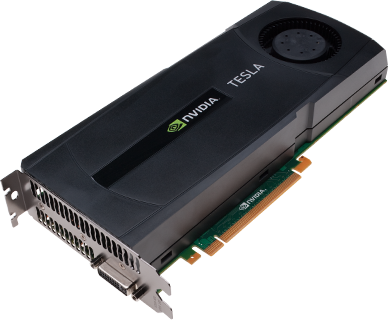
\includegraphics[width=0.2\textwidth]{tesla.png}\quad
        }
        \uncover<1,2,4>{
            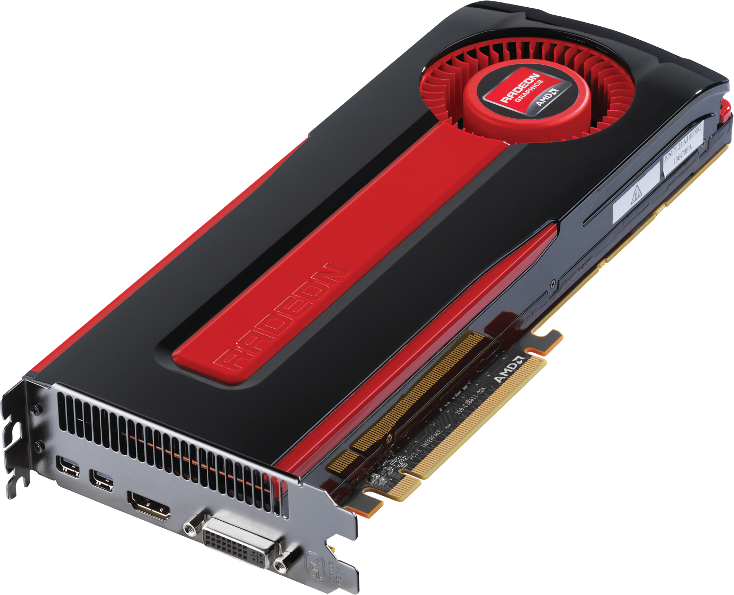
\includegraphics[width=0.2\textwidth]{radeon.png}\quad
        }
        \uncover<1,3>{
            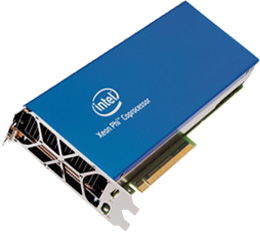
\includegraphics[width=0.17\textwidth]{intel.png}
        }
    \end{figure}
\end{frame}

\note[itemize]{
\item VexCL can transparently work with several compute devices that are
    present on your system.
\item We initialize the VexCL context with a device filter. The device filter
    is a simple functor that acts on device reference and returns a boolean
    value. Several standard filters are provided and you can write your own
    filters.
\item Let's assume that we have an NVIDIA GPU, an AMD GPU, and an Intel CPU
    installed.
    \begin{enumerate}
        \item The standard 'All' Filter select any device available, so we end
            with three devices in our context.
        \item If we want to select only GPUs, then we can filter the devices by
            type.
        \item It is also possible to combine the device filters with logical
            operators.  Here we select a GPU that is provided by AMD OpenCL
            platform.
        \item And here is an example of a custom filter. Here it selects any
            device that has at least 4GB of memory.
    \end{enumerate}
}

\subsection{Распределение нагрузки между картами}

%----------------------------------------------------------------------------
\begin{frame}[fragile]{Распределение памяти и вычислений между картами}
    \setbeamercovered{transparent=40}
    \begin{exampleblock}{}
        \begin{onlyenv}<1|handout:0>
        \begin{lstlisting}
vex::Context ctx( vex::Filter::Name("Tesla") );
        \end{lstlisting}
        \end{onlyenv}
        \begin{onlyenv}<2|handout:0>
        \begin{lstlisting}
vex::Context ctx( vex::Filter::Type(CL_DEVICE_TYPE_GPU) );
        \end{lstlisting}
        \end{onlyenv}
        \begin{onlyenv}<3>
        \begin{lstlisting}
vex::Context ctx( vex::Filter::DoublePrecision );
        \end{lstlisting}
        \end{onlyenv}
        \begin{uncoverenv}<1>
        \begin{lstlisting}[firstnumber=last]

vex::vector<double> x(ctx, N);
vex::vector<double> y(ctx, N);

x = vex::element_index() * (1.0 / N);
y = sin(2 * x) + sqrt(1 - x * x);
        \end{lstlisting}
        \end{uncoverenv}
    \end{exampleblock}
    \setbeamercovered{invisible}
    \begin{figure}
        \begin{tikzpicture}
            \draw (0,2.5) rectangle +(8,0.1);
            \draw (0,2.5) grid[step=0.1] +(8,0.1);
            \draw (-0.3,2.6) node{x};

            \draw (0,2.0) rectangle +(8,0.1);
            \draw (0,2.0) grid[step=0.1] +(8,0.1);
            \draw (-0.3,2.1) node[anchor=center]{y};

            \uncover<1-3> {
            \draw (1,0.5) node{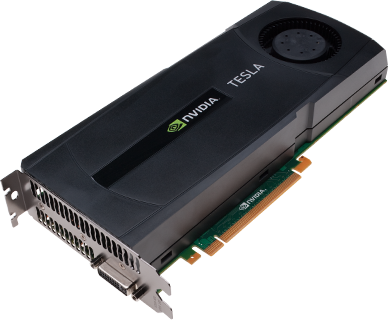
\includegraphics[width=0.2\textwidth]{tesla.png}};
            }

            \uncover<2-3> {
            \draw (4,0.5) node{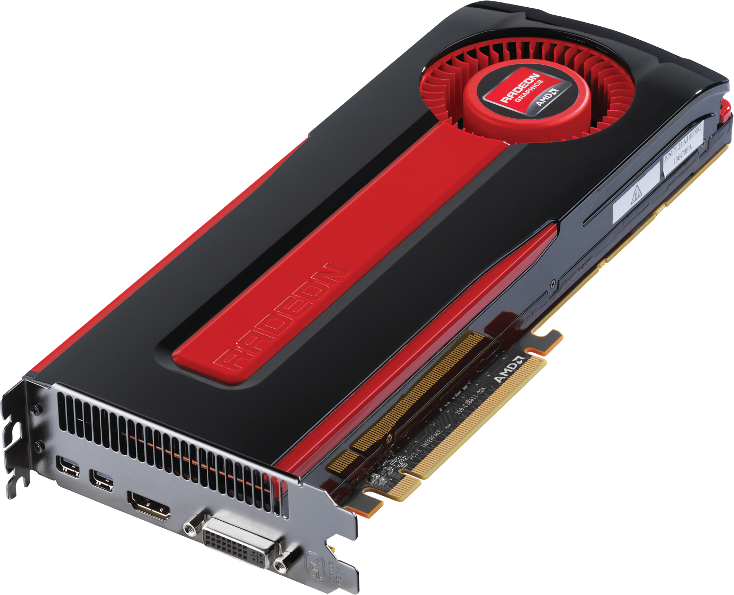
\includegraphics[width=0.2\textwidth]{radeon.png}};
            }

            \uncover<3> {
            \draw (7.5,0.5) node{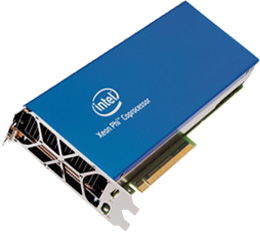
\includegraphics[width=0.17\textwidth]{intel.png}};
            }

            \uncover<1|handout:0> {
            \draw[->,chameleon3,style=dashed] (0,2.7) -- (0,1.8)
                .. controls +(east:0.5) and +(north west:0.5) ..
                (1.4,1.5);
            \draw[->,chameleon3,style=dashed] (8,2.7) -- (8,1.8)
                .. controls +(west:0.5) and +(north east:0.5) ..
                (1.6,1.5);
            }

            \uncover<2|handout:0> {
            \draw[->,chameleon3,style=dashed] (0,2.7) -- (0,1.8)
                .. controls +(east:0.5) and +(north west:0.5) ..
                (1.4,1.5);
            \draw[->,chameleon3,style=dashed] (4,2.7) -- (4,1.8)
                .. controls +(west:0.5) and +(north east:0.5) ..
                (1.6,1.5);

            \draw[->,chameleon3,style=dashed] (4,2.7) -- (4,1.8)
                .. controls +(east:0.1) and +(north west:0.2) ..
                (4.4,1.5);
            \draw[->,chameleon3,style=dashed] (8,2.7) -- (8,1.8)
                .. controls +(west:0.5) and +(north east:0.5) ..
                (4.6,1.5);
            }

            \uncover<3> {
            \draw[->,chameleon3,style=dashed] (0,2.7) -- (0,1.8)
                .. controls +(east:0.5) and +(north west:0.5) ..
                (1.4,1.5);
            \draw[->,chameleon3,style=dashed] (3,2.7) -- (3,1.8)
                .. controls +(west:0.5) and +(north east:0.5) ..
                (1.6,1.5);

            \draw[->,chameleon3,style=dashed] (3,2.7) -- (3,1.8)
                .. controls +(east:0.5) and +(north west:0.2) ..
                (4.4,1.5);
            \draw[->,chameleon3,style=dashed] (6,2.7) -- (6,1.8)
                .. controls +(west:0.5) and +(north east:0.5) ..
                (4.6,1.5);

            \draw[->,chameleon3,style=dashed] (6,2.7) -- (6,1.8) -- (7.4,1.5);
            \draw[->,chameleon3,style=dashed] (8,2.7) -- (8,1.8) -- (7.6,1.5);
            }
        \end{tikzpicture}
    \end{figure}
\end{frame}

\note[itemize]{
\item Now that we know how to initialize VexCL context, let's see how device
    vectors are allocated.
\item Here we allocate three vectors, and initialize two of them with
    constant values.
\item Each vector receives a list of queues at initialization.  Since each
    queue corresponds to a specific device, vectors know where to put their
    data to.
    \begin{enumerate}
        \item For example, if we only have the Tesla card in our context, then
            it will hold the complete memory for all of our vectors.
        \item If we use both of the available GPUs, then the vectors will be
            split between the devices. This split is by default proportional to
            the GPU bandwidth and is guaranteed to be consistent for vectors of
            the same size. This consistency allows VexCL to run computations
            independently on all devices in context.
        \item If we add the CPU to the context, it will get smaller share of
            the data and arithmetic operations.
    \end{enumerate}
\item Care must be taken with the use of several devices. VexCL tries to split
    the memory as fair as it can, but it is probable that your program will
    run at the speed of the slowest device.
}

\subsection{Перенос данных}

%----------------------------------------------------------------------------
\begin{frame}[fragile]{Перенос данных}
    \begin{exampleblock}{}
        \begin{lstlisting}
vex::vector<double> d(ctx, n);
std::vector<double> h(n);
double a[100];
        \end{lstlisting}
    \end{exampleblock}
    \vspace{\baselineskip}
    \begin{columns}
        \begin{column}{0.5\textwidth}
            \begin{exampleblock}{Копирование диапазонов}
                \begin{lstlisting}
vex::copy(d.begin(), d.end(), h.begin());
vex::copy(d.begin(), d.begin() + 100, a);
                \end{lstlisting}
            \end{exampleblock}
        \end{column}
        \begin{column}{0.4\textwidth}
            \begin{exampleblock}{Простые копии}
                \begin{lstlisting}
vex::copy(d, h);
vex::copy(h, d);
                \end{lstlisting}
            \end{exampleblock}
        \end{column}
    \end{columns}
    \vspace{\baselineskip}
    \begin{columns}
        \begin{column}{0.5\textwidth}
            \begin{exampleblock}{Отображение буффера OpenCL на хостовый указатель}
                \begin{lstlisting}
auto p = d.map(devnum);
std::sort(&p[0], &p[d.part_size(devnum)]);
                \end{lstlisting}
            \end{exampleblock}
        \end{column}
        \begin{column}{0.4\textwidth}
            \begin{exampleblock}{Доступ к единственному элементу
                (\emph{медленно})}
                \begin{lstlisting}
double v = d[42];
d[0] = 0;
                \end{lstlisting}
            \end{exampleblock}
        \end{column}
    \end{columns}
\end{frame}

\note[itemize]{
\item Copies between host and device memory may be done with simple copy
    function that copy the complete vector either way,
\item or, if you need to do partial copy, you can use STL-like syntax.
\item Vectors also overload array subscript operator, so you can have direct
    read or write access to any element of a vector. But this should be used
    with caution because it is slow. The intended use for this is a single
    element access or debugging.
\item Data may also be accessed through iterators, so it is possible to use,
    for example, an STL algorithm with device vector as a temporary solution.
}

\subsection{Векторные выражения}

%----------------------------------------------------------------------------
\begin{frame}[fragile]{Язык векторных выражений VexCL}
    \begin{itemize}
        \item Все векторы в выражении должны быть \emph{совместимыми}:
            \begin{itemize}
                \item Иметь один размер
                \item Быть расположенными на одних и тех же устройствах
            \end{itemize}
        \item Что можно использовать в выражениях:
            \begin{columns}
                \begin{column}{0.4\textwidth}
                    \begin{itemize}
                        \item Векторы, скаляры, константы
                        \item Арифм. и логич. операторы
                        \item Встроенные функции
                        \item Пользовательские функции
                        \item Генераторы случайных чисел
                        \item Сортировка, префиксные суммы
                    \end{itemize}
                \end{column}
                \begin{column}{0.4\textwidth}
                    \begin{itemize}
                        \item Временные значения
                        \item Срезы и перестановки
                        \item Редукция (сумма, экстремумы)
                        \item Произв. матрицы на вектор
                        \item Свертки
                        \item Быстрое преобразование Фурье
                    \end{itemize}
                \end{column}
            \end{columns}
    \end{itemize}
\end{frame}

\note[itemize]{
\item So, what kind of expressions can you use in VexCL?
\item First, any vectors used in an expression have to be compatible.
\item If this requirement is satisfied, then expressions may combine
    vectors and scalars with almost any binary operators. OpenCL math functions
    and user-defined functions are also available.
}

%----------------------------------------------------------------------------
\begin{frame}[fragile]{Встроенные операторы и функции}
    \begin{columns}
        \begin{column}{0.38\textwidth}
            \begin{exampleblock}{Выражение:}
                \begin{lstlisting}
x = 2 * y - sin(z);
                \end{lstlisting}
            \end{exampleblock}
        \end{column}
        \begin{column}{0.55\textwidth}
            \begin{itemize}
                \item \code{export VEXCL_SHOW_KERNELS=1}\\
                    чтобы увидеть сгенерированный код.
            \end{itemize}
        \end{column}
    \end{columns}
    \begin{exampleblock}{\ldots генерирует ядро:}
        \begin{lstlisting}
kernel void vexcl_vector_kernel(
    ulong n,
    global double * prm_1,
    int prm_2,
    global double * prm_3,
    global double * prm_4
)
{
    for(size_t idx = get_global_id(0); idx < n; idx += get_global_size(0)) {
        prm_1[idx] = ( ( prm_2 * prm_3[idx] ) - sin( prm_4[idx] ) );
    }
}
        \end{lstlisting}
    \end{exampleblock}
    \begin{tikzpicture}[overlay,scale=0.6]
        \draw (16,8) node(sub)[draw,fill=white,ellipse,drop shadow]{$-$};

        \draw (sub) +(-2.00,-1) node(mul)[draw,fill=white,drop shadow,ellipse]{$*$};
        \draw (sub) +( 2.00,-1) node(sin)[draw,fill=white,drop shadow,ellipse]{sin};
        \draw (mul) +(-2.00,-1) node(two)[draw,fill=white,drop shadow,minimum size=0.5cm]{2};
        \draw (mul) +( 2.00,-1) node(y)  [draw,fill=white,drop shadow,minimum size=0.5cm]{y};
        \draw (sin) +( 1.75,-1) node(z)  [draw,fill=white,drop shadow,minimum size=0.5cm]{z};

        \draw (sub) -- (mul);
        \draw (sub) -- (sin);
        \draw (mul) -- (two);
        \draw (mul) -- (y);
        \draw (sin) -- (z);
    \end{tikzpicture}
\end{frame}

\note{ }

%----------------------------------------------------------------------------
\begin{frame}[fragile]{Индексы элементов}
    \begin{itemize}
        \item \code{vex::element_index(size_t offset = 0, size_t size = 0)}\\
            возвращает индекс текущего элемента вектора.
            \begin{itemize}
                \item Нумерация начинается с \code{offset}, элементы на всех
                    устройствах нумеруются последовательно.
                \item Необязательный параметр \code{size} задает размер
                    выражения.
            \end{itemize}
    \end{itemize}
    \begin{exampleblock}{Линейная функция:}
        \begin{lstlisting}
vex::vector<double> X(ctx, N);
double x0 = 0, dx = 1e-3;
X = x0 + dx * vex::element_index();
        \end{lstlisting}
    \end{exampleblock}
    \begin{exampleblock}{Один период функции синуса:}
        \begin{lstlisting}
X = sin(2 * M_PI / N * vex::element_index());
        \end{lstlisting}
    \end{exampleblock}
\end{frame}

\note[itemize]{
\item \code{element_index} is a function that allows you to use element
    position inside of vector expressions.
\item The function may participate in arbitrary vector expressions.
\item For example, here\ldots
}

%----------------------------------------------------------------------------
\begin{frame}[fragile]{Пользовательские функции}
    \begin{exampleblock}{Определение функции:}
        \begin{lstlisting}
VEX_FUNCTION( double, sqr, (double, x)(double, y),
    return x * x + y * y;
    );
        \end{lstlisting}
    \end{exampleblock}
    \begin{exampleblock}{Использование функции:}
        \begin{lstlisting}
Z = sqrt( sqr(X, Y) );
        \end{lstlisting}
    \end{exampleblock}
\end{frame}

\note[itemize]{
\item It is possible to define an OpenCL function that may be used with vector
    expressions. You need to provide function body, parameter types, and return
    type.
\item Function body has to be of \code{extern const char} type, to allow its
    use as a template parameter. And it has to be defined at global scope.
\item Inside the body function parameters are always named prm1, prm2, etc.
\item Here we define 'between' function that returns true if its second
    parameter is between its first and third parameters. The UserFunction
    object is stateless, so it may be good idea to define it at global scope
    as well, next to its body.
\item Now we may use the function in expressions. Any vector expression may be
    used as a parameter for a user-defined (or builtin) function.
}

%----------------------------------------------------------------------------
\begin{frame}[fragile]{Пользовательские функции транслируются в функции OpenCL}
    \begin{exampleblock}{}
        \begin{lstlisting}
Z = sqrt( sqr(X, Y) );
        \end{lstlisting}
    \end{exampleblock}
    \begin{exampleblock}{\ldots ведет к генерации ядра:}
        \begin{lstlisting}
double sqr(double x, double y) {
    return x * x + y * y;
}

kernel void vexcl_vector_kernel(
    ulong n,
    global double * prm_1,
    global double * prm_2,
    global double * prm_3
)
{
    for(size_t idx = get_global_id(0); idx < n; idx += get_global_size(0)) {
        prm_1[idx] = sqrt( sqr( prm_2[idx], prm_3[idx] ) );
    }
}
        \end{lstlisting}
    \end{exampleblock}
    \begin{tikzpicture}[overlay,scale=0.6]
        \draw (16,8.75) node(sqrt)[draw,fill=white,ellipse,drop shadow]{sqrt};

        \draw (sqrt) +(0.00,-2) node(sqr)[draw,fill=white,ellipse,drop shadow]{sqr};

        \draw (sqr) +(-2.00,-1) node(x) [draw,fill=white,drop shadow,minimum size=0.5cm]{x};
        \draw (sqr) +( 2.20,-1) node(y) [draw,fill=white,drop shadow,minimum size=0.5cm]{y};

        \draw (sqrt) -- (sqr);
        \draw (sqr)  -- (x);
        \draw (sqr)  -- (y);
    \end{tikzpicture}
\end{frame}

\note{ }

%----------------------------------------------------------------------------
\begin{frame}[fragile]{Функции часто не только удобны, но и эффективны}
    \begin{exampleblock}{Тот же пример без использования функции:}
        \begin{lstlisting}
Z = sqrt( X * X + Y * Y );
        \end{lstlisting}
    \end{exampleblock}
    \begin{exampleblock}{\ldots транслируется в:}
        \begin{lstlisting}
kernel void vexcl_vector_kernel(
  ulong n,
  global double * prm_1,
  global double * prm_2,
  global double * prm_3,
  global double * prm_4,
  global double * prm_5
)
{
  for(size_t idx = get_global_id(0); idx < n; idx += get_global_size(0)) {
    prm_1[idx] = sqrt( ( ( prm_2[idx] * prm_3[idx] ) + ( prm_4[idx] * prm_5[idx] ) ) );
  }
}
        \end{lstlisting}
    \end{exampleblock}
    \begin{tikzpicture}[overlay,scale=0.6]
        \draw (16,8.75) node(sqrt)[draw,fill=white,ellipse,drop shadow]{sqrt};

        \draw (sqrt) +(0.00,-2) node(sum)[draw,fill=white,ellipse,drop shadow]{$+$};

        \draw (sum) +(-3.00,-1) node(mul1)[draw,fill=white,drop shadow,ellipse]{$*$};
        \draw (sum) +( 3.00,-1) node(mul2)[draw,fill=white,drop shadow,ellipse]{$*$};

        \draw (mul1) +(-2.00,-1) node(x1) [draw,fill=white,drop shadow,minimum size=0.5cm]{x};
        \draw (mul1) +( 2.00,-1) node(x2) [draw,fill=white,drop shadow,minimum size=0.5cm]{x};

        \draw (mul2) +(-2.00,-1) node(y1) [draw,fill=white,drop shadow,minimum size=0.5cm]{y};
        \draw (mul2) +( 2.00,-1) node(y2) [draw,fill=white,drop shadow,minimum size=0.5cm]{y};

        \draw (sqrt) -- (sum);
        \draw (sum)  -- (mul1);
        \draw (sum)  -- (mul2);
        \draw (mul1) -- (x1);
        \draw (mul1) -- (x2);
        \draw (mul2) -- (y1);
        \draw (mul2) -- (y2);
    \end{tikzpicture}
\end{frame}

\note{ }

%----------------------------------------------------------------------------
\begin{frame}[fragile]{Повторное использование промежуточных результатов}
    \begin{columns}
        \begin{column}{0.48\textwidth}
            \begin{itemize}
                \item Некоторые выражения используют промежуточные результаты
                    несколько раз:
            \end{itemize}
            \begin{exampleblock}{}
                \begin{lstlisting}
Z = log(X) * (log(X) + Y);
                \end{lstlisting}
            \end{exampleblock}
            \begin{itemize}
                \item \code{log(X)} будет вычислен дважды.
                \item В простых случаях компилятор сможет избавиться от
                    избыточного кода\ldots
            \end{itemize}
        \end{column}
        \begin{column}{0.48\textwidth}
            \begin{tikzpicture}
                \draw (0,0) node(mul)[draw,fill=white,ellipse,drop shadow,minimum size=0.8cm]{$*$};
                \draw (mul)  +( 1.50,-1) node(sum)  [draw,fill=white,ellipse,drop shadow,minimum size=0.8cm]{$+$};
                \draw (mul)  +(-1.50,-1) node(log1) [draw,fill=chameleon2!50,ellipse,drop shadow,minimum size=0.5cm]{log};
                \draw (sum)  +(-1.50,-1) node(log2) [draw,fill=chameleon2!50,ellipse,drop shadow,minimum size=0.5cm]{log};
                \draw (log1) +( 0.00,-1) node(x1)   [draw,fill=chameleon2!50,drop shadow,minimum size=0.5cm]{x};
                \draw (log2) +( 0.00,-1) node(x2)   [draw,fill=chameleon2!50,drop shadow,minimum size=0.5cm]{x};
                \draw (sum)  +( 1.50,-1) node(y)    [draw,fill=white,drop shadow,minimum size=0.5cm]{y};

                \draw (mul)  -- (log1);
                \draw (mul)  -- (sum);
                \draw (log1) -- (x1);
                \draw (sum)  -- (log2);
                \draw (sum)  -- (y);
                \draw (log2) -- (x2);
            \end{tikzpicture}
        \end{column}
    \end{columns}
\end{frame}

\note{ }

%----------------------------------------------------------------------------
\begin{frame}[fragile]{Промежуточные значения}
    \begin{itemize}
        \item VexCL позволяет явно сохранить и использовать промежуточный
            результат:
    \end{itemize}
    \begin{exampleblock}{}
        \begin{lstlisting}
auto tmp = vex::make_temp<1>( log(X) );
Z = tmp * (tmp + Y);
        \end{lstlisting}
    \end{exampleblock}
    \begin{exampleblock}{}
        \begin{lstlisting}
kernel void vexcl_vector_kernel(
    ulong n,
    global double * prm_1,
    global double * prm_2,
    global double * prm_3
)
{
    for(size_t idx = get_global_id(0); idx < n; idx += get_global_size(0)) {
        double temp_1 = log( prm_2[idx] );
        prm_1[idx] = ( temp_1 * ( temp_1 + prm_3[idx] ) );
    }
}
        \end{lstlisting}
    \end{exampleblock}
\end{frame}

\note{ }

%----------------------------------------------------------------------------
\begin{frame}[fragile]{Перестановки} \singledevice
    \begin{itemize}
        \item \code{vex::permutation(expr)} принимает произвольное
            целочисленное выражение и возвращает функтор:
            \begin{exampleblock}{}
                \begin{lstlisting}
auto reverse = vex::permutation(N - 1 - vex::element_index(0, N));
y = reverse(x);
                \end{lstlisting}
            \end{exampleblock}
        \item Перестановки поддерживают как чтение, так и запись:
            \begin{exampleblock}{}
                \begin{lstlisting}
reverse(y) = x;
                \end{lstlisting}
            \end{exampleblock}
    \end{itemize}

    \begin{exampleblock}{Пример: выделение вещественной и мнимой частей вектора}
        \begin{lstlisting}
vex::vector<double> x(ctx, n * 2), y(ctx, n);

auto Re = vex::permutation(2 * vex::element_index(0, n));
auto Im = vex::permutation(2 * vex::element_index(0, n) + 1);

y = sqr(Re(x), Im(x));
        \end{lstlisting}
    \end{exampleblock}
\end{frame}

\note{ }

\subsection{Срезы многомерных массивов}

%----------------------------------------------------------------------------
\begin{frame}[fragile]{Срезы многомерных массивов} \singledevice
    \begin{itemize}
        \item При работе с многомерными массивами данные эффективнее всего
            располагать в непрерывных одномерных массивах.
            \begin{itemize}
                \item Класс \code{vex::slicer<NDIM>} позволяет работать со
                    срезами таких массивов.
            \end{itemize}
    \end{itemize}
    \begin{exampleblock}{Матрица NxN и slicer:}
        \begin{lstlisting}
vex::vector<double> x(ctx, n * n);
vex::slicer<2> slice(vex::extents[n][n]);
        \end{lstlisting}
    \end{exampleblock}
    \pause
    \begin{exampleblock}{Доступ к строке или столбцу матрицы:}
        \begin{lstlisting}[firstnumber=last]
using vex::_;
y = slice[42](x);       // строка
y = slice[_][42](x);    // столбец
slice[_][10](x) = y;
        \end{lstlisting}
    \end{exampleblock}
    \pause
    \begin{exampleblock}{Использование диапазонов для выделения подблоков:}
        \begin{lstlisting}[firstnumber=last]
z = slice[vex::range(0, 2, n)][vex::range(10, 20)](x);
        \end{lstlisting}
    \end{exampleblock}
\end{frame}

\note{ }

\begin{frame}[fragile]{Тензорное произведение}
    \begin{description}[\;\;]
        \item[Тензорное произведение] --- обобщенная версия скалярного
            произведения.  Элементы двух многомерных массивов перемножаются и
            суммируются вдоль заданных осей.
    \end{description}
    \begin{exampleblock}{Произведение матрицы на вектор}
        \begin{lstlisting}
vex::vector<double> A(ctx, n * m), x(ctx, m), y(ctx, n);
vex::slicer<2> Adim(vex::extents[n][m]);
vex::slicer<1> xdim(vex::extents[m]);

y = vex::tensordot(Adim[_](A), xdim[_](x), vex::axes_pairs(1, 0));
        \end{lstlisting}
    \end{exampleblock}
    \begin{exampleblock}{Произведение двух матриц}
        \begin{lstlisting}
vex::vector<double> A(ctx, n * m), B(ctx, m * k), C(ctx, n * k);
vex::slicer<2> Adim(vex::extents[n][m]);
vex::slicer<1> Bdim(vex::extents[m][k]);

C = vex::tensordot(Adim[_](A), Bdim[_](B), vex::axes_pairs(1, 0));
        \end{lstlisting}
    \end{exampleblock}
\end{frame}

%----------------------------------------------------------------------------
\begin{frame}[fragile]{Генерация случайных чисел}
    \begin{itemize}
        \item В VexCL реализованы позиционные генераторы случайных
            чисел\footnote{Random123 suite, D. E. Shaw Research,
            \href{http://www.deshawresearch.com/resources\_random123.html}{deshawresearch.com/resources\_random123.html}}
            (Counter-Based RNG)
            \begin{itemize}
                \item Такие генераторы не имеют состояния и позволяют\\
                    получить случайное число по его номеру (позиции) за O(1).
                \item Реализованные семейства: \code{threefry} и \code{philox}.
                \item Удовлетворяют тестам TestU01/BigCrush; позволяют
                    получить\\ до \alert{$2^{64}$} независимых
                    последовательностей с периодом \alert{$2^{128}$}.
                \item Производительность: \alert{$\approx
                    2\times10^{10}$}~чисел/сек (Tesla K40c).
            \end{itemize}
        \item \code{vex::Random<T, G=philox>}~--- равномерное распределение.
        \item \code{vex::RandomNormal<T, G=philox>}~--- нормальное распределение.
    \end{itemize}
    \begin{exampleblock}{}
        \begin{lstlisting}
vex::Random<double> rnd;
vex::vector<double> x(ctx, n);

x = rnd(vex::element_index(), std::rand());
        \end{lstlisting}
    \end{exampleblock}
\end{frame}

\note[itemize]{
\item Random number generation is a useful feature that is used often in, e.g.,
    molecular dynamics.
\item Random number generators in VexCL are stateless, so they don't require
    additional storage or global memory interactions. Randomness is obtained by
    applying mixing functions to element indices.
}

\subsection{Редукция}

%----------------------------------------------------------------------------
\begin{frame}[fragile]{Редукция}
    \begin{itemize}
        \item Класс \code{vex::Reductor<T, kind=SUM>} позволяет редуцировать
            произвольное \emph{векторное выражение} и получить значение типа
            \code{T}.
        \item Виды редукции: \code{SUM}, \code{SUM_Kahan}, \code{MIN},
            \code{MAX}
    \end{itemize}
    \begin{exampleblock}{Скалярное произведение}
        \begin{lstlisting}
vex::Reductor<double> sum(ctx);
double s = sum(x * y);
        \end{lstlisting}
    \end{exampleblock}
    \begin{exampleblock}{Число элементов в интервале (0, 1)}
        \begin{lstlisting}
vex::Reductor<size_t> sum(ctx);
size_t n = sum( (x > 0) && (x < 1) );
        \end{lstlisting}
    \end{exampleblock}
    \begin{exampleblock}{Максимальное расстояние от центра}
        \begin{lstlisting}
vex::Reductor<double, vex::MAX> max(ctx);
double d = max( sqrt(x * x + y * y) );
        \end{lstlisting}
    \end{exampleblock}
\end{frame}

\note[itemize]{
\item Reduction is an operation of reducing a vector to a single value.
\item The most frequent types are summation and finding minimum or maximum
    element of a vector.
\item VexCL provides Reductor functor that accepts any valid vector expression
    as a parameter.
\item For example, to compute an inner product of two vectors we compute sum of
    their elementwise product.
\item To find number of elements in vector x that are greater than zero and
    less than one, we compute sum of the corresponding boolean expression.
\item And to find the maximum distance from axis origin for a set of
    two-dimensional points, we compute exactly that: max of their radius.
}

%----------------------------------------------------------------------------
\begin{frame}[fragile]{Пример: число $\pi$ методом Монте-Карло}
    \vspace{-1\baselineskip}
    \begin{columns}
        \begin{column}{0.55\textwidth}
            \begin{itemize}
                \item Приближенная оценка $\pi$:
            \end{itemize}
            \vspace{\baselineskip}
            \begin{equation*}
                \frac{\text{площадь круга}}{\text{площадь квадрата}} =
                \frac{\pi r^2}{(2r)^2} = \frac{\pi}{4},
            \end{equation*}
            \begin{equation*}
                \pi = 4 \frac{\text{площадь круга}}{\text{площадь квадрата}}
                \approx 4 \frac{\text{\color{chameleon2}{точки в
                круге}}}{\text{\color{chameleon2}{все}
                \color{chameleon3}{точки}}}
            \end{equation*}
        \end{column}
        \begin{column}{0.35\textwidth}
            \begin{figure}
                \includegraphics[width=\textwidth]{mcpi}
            \end{figure}
        \end{column}
    \end{columns}
    \begin{exampleblock}{}
        \begin{lstlisting}[texcl=true]
vex::Random<cl_double2> rnd;
vex::Reductor<size_t, vex::SUM> sum(ctx);

double pi = 4.0 * sum( length( rnd(vex::element_index(0, n), seed) ) < 1 ) / n;
        \end{lstlisting}
    \end{exampleblock}
\end{frame}

\note[itemize]{
\item Here is a bit more complex example of what you can do with VexCL.
\item Imagine we want to compute an approximate value of $\pi$ with Monte-Carlo
    method. We can use the following equalities to do this.
}

%----------------------------------------------------------------------------
\begin{frame}[fragile]{Монте-Карло $\pi$: сгенерированное ядро}
    \begin{columns}
        \begin{column}[t]{0.2\textwidth}
            \begin{exampleblock}{}
                \begin{adjustbox}{width=0.23\textwidth, height=\textheight, keepaspectratio}
                    \begin{minipage}{\textwidth}
                        \lstinputlisting[linerange={1-49}]{code/pi-kernel.cpp}
                    \end{minipage}
                \end{adjustbox}
            \end{exampleblock}
        \end{column}
        \begin{column}[t]{0.2\textwidth}
            \begin{exampleblock}{}
                \begin{adjustbox}{width=0.23\textwidth, height=\textheight, keepaspectratio}
                    \begin{minipage}{\textwidth}
                        \lstinputlisting[firstnumber=last,linerange={50-98}]{code/pi-kernel.cpp}
                    \end{minipage}
                \end{adjustbox}
            \end{exampleblock}
        \end{column}
        \begin{column}[t]{0.2\textwidth}
            \begin{exampleblock}{}
                \begin{adjustbox}{width=0.23\textwidth, height=\textheight, keepaspectratio}
                    \begin{minipage}{\textwidth}
                        \lstinputlisting[firstnumber=last,linerange={99-147}]{code/pi-kernel.cpp}
                    \end{minipage}
                \end{adjustbox}
            \end{exampleblock}
        \end{column}
        \begin{column}[t]{0.3\textwidth}
            \begin{exampleblock}{}
                \begin{adjustbox}{width=0.23\textwidth, height=\textheight, keepaspectratio}
                    \begin{minipage}{\textwidth}
                        \lstinputlisting[firstnumber=last,linerange={148-196}]{code/pi-kernel.cpp}
                        \vspace{\baselineskip}
                    \end{minipage}
                \end{adjustbox}
            \end{exampleblock}
        \end{column}
    \end{columns}
\end{frame}

\note{}

%----------------------------------------------------------------------------
\begin{frame}[fragile]{Произведение разреженной матрицы на вектор} \additive
    \begin{itemize}
        \item Класс \code{vex::SpMat<T>} содержит представление разреженной
            матрицы на вычислительных устройствах.
        \item Конструктор принимает матрицу в формате CRS:
            \begin{itemize}
                \item Номера столбцов и значения ненулевых элементов, указатели
                    на начало каждой строки.
            \end{itemize}
    \end{itemize}
    \begin{exampleblock}{Конструирование матрицы}
        \begin{lstlisting}
vex::SpMat<double> A(ctx, n, n, row.data(), col.data(), val.data());
        \end{lstlisting}
    \end{exampleblock}

    \begin{exampleblock}{Расчет невязки СЛАУ}
        \begin{lstlisting}[firstnumber=last]
vex::vector<double> u, f, r;
r = f - A * u;
double res = max( fabs(r) );
        \end{lstlisting}
    \end{exampleblock}
\end{frame}

\note[itemize]{
\item Sparse matrix -- vector operation is also provided. A matrix is imported
    from commonly used compressed row storage format.
\item Note that matrix-vector product is not a first-class citizen in vector
    expressions. It uses neighbor values; and neighbors may reside on a
    different compute device. So extra work is needed to exchange data between
    devices. That is why matrix-vector products may only be used in additive
    expressions.
}

%----------------------------------------------------------------------------
\begin{frame}[fragile]{Арифметика указателей} \singledevice
    \begin{itemize}
        \item Функция \code{raw_pointer(const vector<T>&)} возвращает указатель
            на данные вектора.
            \begin{itemize}
                \item Может использоваться для реализации случайного доступа
            \end{itemize}
    \end{itemize}
    \begin{exampleblock}{Одномерный оператор Лапласа:}
        \begin{lstlisting}
VEX_FUNCTION(double, laplace, (size_t, i)(size_t, n)(double*, x),
    if (i == 0 || i == n-1) return 0;
    return 2 * x[i] - x[i-1] - x[i+1];
    );

y = laplace(vex::element_index(), n, vex::raw_pointer(x));
        \end{lstlisting}
    \end{exampleblock}
\end{frame}

\note{ }

%----------------------------------------------------------------------------
\begin{frame}[fragile]{Пример: взаимодействие N тел}
    \begin{equation*}
        y_i = \sum_{j \neq i} e^{-|x_i - x_j|}
    \end{equation*}
    \begin{exampleblock}{}
        \begin{lstlisting}
VEX_FUNCTION(double, nbody, (size_t, i)(size_t, n)(double*, x),
    double sum = 0, myval = x[i];
    for(size_t j = 0; j < n; ++j)
        if (j != i) sum += exp(-fabs(x[j] - myval));
    return sum;
    );

y = nbody(vex::element_index(), x.size(), raw_pointer(x));
        \end{lstlisting}
    \end{exampleblock}
\end{frame}

\note{ }

\subsection{Fast Fourier Transform}

%----------------------------------------------------------------------------
\begin{frame}[fragile]{Быстрое преобразование Фурье \singledevice}
    \begin{itemize}
        \item Произвольное выражение на входе
        \item Многомерные преобразования
        \item Произвольные размеры массивов
        \item В 2-3 медленнее Nvidia CUFFT, сравнимо по скорости с AMD clFFT
    \end{itemize}
    \begin{exampleblock}{Решение периодической задачи Пуассона:}
        \begin{lstlisting}
vex::vector<double> rhs(ctx, n), u(ctx, n), K(ctx, n);

vex::FFT<double, cl_double2> fft(ctx, n);
vex::FFT<cl_double2, double> ifft(ctx, n, vex::inverse);

u = ifft( K * fft(rhs) );
        \end{lstlisting}
    \end{exampleblock}
\end{frame}

\note{ }

\subsection{Мультивекторы и мультивыражения}

%----------------------------------------------------------------------------
\begin{frame}[fragile]{Мультивекторы}
    \begin{itemize}
        \item Класс \code{vex::multivector<T,N>} владеет \code{N} экземплярами
            класса \code{vex::vector<T>} одного размера.
        \item Поддерживает все операции, определенные для
            \code{vex::vector<T>}.
        \item Операции с мультивекторами выполняются в единственном ядре.
        \item \code{vex::multivector::operator()(size_t k)} возвращает
            \code{k}-ю компоненту.
    \end{itemize}
    \begin{exampleblock}{}
        \begin{lstlisting}
vex::multivector<double, 2> X(ctx, N), Y(ctx, N);
vex::Reductor<double, vex::SUM> sum(ctx);
vex::SpMat<double> A(ctx, ... );
std::array<double, 2> v;

X = sin(v * Y + 1);             // X(k) = sin(v[k] * Y(k) + 1);
v = sum( between(0, X, Y) );    // v[k] = sum( between( 0, X(k), Y(k) ) );
X = A * Y;                      // X(k) = A * Y(k);
        \end{lstlisting}
    \end{exampleblock}
\end{frame}

\note[itemize]{
\item This is in principle all of the basic VexCL operations.
\item What is left are multivectors and multiexpressions.
}

%----------------------------------------------------------------------------
\begin{frame}[fragile]{Мультивыражения}
    \begin{itemize}
        \item Некоторые операции не удается выразить через арифметику
            мультивекторов.
    \end{itemize}
    \begin{block}{Пример: вращение 2D вектора на заданный угол}
        \vspace{-1\baselineskip}
        \begin{align*}
            y_0 &= x_0 \cos \alpha - x_1 \sin \alpha, \\
            y_1 &= x_0 \sin \alpha + x_1 \cos \alpha.
        \end{align*}
    \end{block}

    \begin{itemize}
        \item Мультивыражение --- это кортеж (tuple) векторых выражений.
        \item Присваивание мультивыражения мультивектору эквивалентно
            покомпонентному присваиванию, но выполняется в единственном ядре.
    \end{itemize}
\end{frame}

\note[itemize]{
\item Sometimes it's not possible to express the required operation with simple
    multivector arithmetics.
\item For example, take two-dimensional point rotation operation, which is
    defined as this couple of expressions. X and Y coordinates are mixed
    here, so we either have to split the operation in two, or use a
    multiexpression.
}

%----------------------------------------------------------------------------
\begin{frame}[fragile]{}
    \begin{itemize}
        \item Мультивыражения можно присваивать мультивекторам:
    \end{itemize}
    \begin{exampleblock}{}
        \begin{lstlisting}
// double alpha;
// vex::multivector<double,2> X, Y;

Y = std::tie( X(0) * cos(alpha) - X(1) * sin(alpha),
              X(0) * sin(alpha) + X(1) * cos(alpha)  );
        \end{lstlisting}
    \end{exampleblock}
    \begin{itemize}
        \item и кортежу выражений:
    \end{itemize}
    \begin{exampleblock}{}
        \begin{lstlisting}
// vex::vector<double> alpha;
// vex::vector<double> odlX, oldY, newX, newY;

vex::tie(newX, newY) = std::tie( oldX * cos(alpha) - oldY * sin(alpha),
                                  oldX * sin(alpha) + oldY * cos(alpha)  );
        \end{lstlisting}
    \end{exampleblock}
\end{frame}

\note[itemize]{
\item You can assign a tuple of expressions to a multivector, or to a tuple of
    single vectors.
\item In either case, this will result in single kernel launch that will update
    all parts of the result at once.
\item Also note that in the second example we rotate every point by its own
    angle stored in alpha vector.
}

%----------------------------------------------------------------------------
\begin{frame}[fragile,shrink=5]{Мультивыражение транслируется в единственное
    ядро}
    \begin{exampleblock}{}
        \begin{lstlisting}
auto x0 = tag<0>( X(0) );
auto x1 = tag<1>( X(1) );
auto ca = tag<2>( cos(alpha) );
auto sa = tag<3>( sin(alpha) );

Y = std::tie(x0 * ca - x1 * sa, x0 * sa + x1 * ca);
        \end{lstlisting}
    \end{exampleblock}
    \begin{exampleblock}{}
        \begin{lstlisting}
kernel void vexcl_multivector_kernel(ulong n,
    global double * lhs_1, global double * lhs_2,
    global double * rhs_1, double rhs_2,
    global double * rhs_3, double rhs_4
)
{
    for(size_t idx = get_global_id(0); idx < n; idx += get_global_size(0)) {
        double buf_1 = ( ( rhs_1[idx] * rhs_2 ) - ( rhs_3[idx] * rhs_4 ) );
        double buf_2 = ( ( rhs_1[idx] * rhs_4 ) + ( rhs_3[idx] * rhs_2 ) );

        lhs_1[idx] = buf_1;
        lhs_2[idx] = buf_2;
    }
}

        \end{lstlisting}
    \end{exampleblock}
\end{frame}

\note{ }

%----------------------------------------------------------------------------
\begin{frame}[fragile]{}
    \begin{itemize}
        \item VexCL позволяет писать компактный и читаемый код
            \begin{itemize}
                \item Хорошо подходит для быстрой разработки научных GPGPU
                    приложений.
                \item Производительность часто сравнима с ядрами, написанными
                    вручную.
            \end{itemize}
    \end{itemize}
    \vspace{\baselineskip}
    \begin{itemize}
        \item[{[1]}] D. Demidov, K. Ahnert, K. Rupp, and P. Gottschling.\\
            Programming CUDA and OpenCL: A Case Study Using Modern \CXX Libraries.\\
            \emph{SIAM J. Sci. Comput.,} 35(5):C453 – C472, 2013.\\
            \href{http://dx.doi.org/10.1137/120903683}{doi:10.1137/120903683}
        \item[{[2]}] K. Ahnert, D. Demidov, and M. Mulansky.\\
            Solving ordinary differential equations on GPUs.\\
            In \emph{Numerical Computations with GPUs} (pp. 125-157).  Springer, 2014.
            \href{http://dx.doi.org/10.1007/978-3-319-06548-9\_7}{doi:10.1007/978-3-319-06548-9\_7}
    \end{itemize}
\end{frame}

\note{ }

%----------------------------------------------------------------------------
\begin{frame}
    \begin{center}
        \huge{Как это работает?}
    \end{center}
\end{frame}

\note{ }

%----------------------------------------------------------------------------
\section{Шаблоны выражений}
\begin{frame}
    \sectionpage
\end{frame}

\note{}

%----------------------------------------------------------------------------
\begin{frame}{Шаблоны выражений}
    \begin{itemize}
        \item Как \emph{эффективно} реализовать предметно-ориентированный язык
            (DSL) в \CXX?
            \vspace{\baselineskip}
        \item Идея не нова:
            \begin{itemize}
                \item \emph{Todd Veldhuizen}, Expression templates, \CXX Report,
                    \alert{1995}
            \end{itemize}
        \item Первая (?) реализация:
            \begin{itemize}
                \item ''Blitz\plusplus~--- это библиотека классов \CXX для
                    научных расчетов, имеющая производительность сравнимую с
                    Фортраном 77/90''.
            \end{itemize}
        \item Сегодня:
            \begin{itemize}
                \item Boost.uBLAS, Blaze, MTL, Eigen, Armadillo, и~пр.
            \end{itemize}
            \vspace{\baselineskip}
        \item \emph{Как это работает?}
    \end{itemize}
\end{frame}

\note{ }

%----------------------------------------------------------------------------
\begin{frame}[fragile]{Простой пример: сложение векторов}
    \begin{exampleblock}{Мы хотим иметь возможность написать:}
        \begin{lstlisting}
x = y + z;
        \end{lstlisting}
    \end{exampleblock}

    \begin{exampleblock}{чтобы результат был так же эффективен как:}
        \begin{lstlisting}
for(size_t i = 0; i < n; ++i)
    x[i] = y[i] + z[i];
        \end{lstlisting}
    \end{exampleblock}
\end{frame}

\note{ }

%----------------------------------------------------------------------------
\begin{frame}[fragile]{\CXX допускает перегрузку операторов!}
    \begin{exampleblock}{}
        \begin{lstlisting}
vector operator+(const vector &a, const vector &b) {
    vector tmp( a.size() );
    for(size_t i = 0; i < a.size(); ++i)
        tmp[i] = a[i] + b[i];
    return tmp;
}
        \end{lstlisting}
    \end{exampleblock}
    \begin{uncoverenv}<2>
        \begin{itemize}
            \item Проблемы:
                \begin{itemize}
                    \item Дополнительное выделение памяти
                    \item Дополнительные операции чтения/записи
                \end{itemize}
        \end{itemize}
        \begin{columns}
            \begin{column}{0.45\textwidth}
                \begin{exampleblock}{}
                    \begin{lstlisting}[aboveskip=0.4\baselineskip,belowskip=0.4\baselineskip]
a = x + y + z;

                    \end{lstlisting}
                \end{exampleblock}
                \begin{itemize}
                    \item 2 временных вектора
                    \item $8 \times \text{n}$ операций чтения/записи
                \end{itemize}
            \end{column}
            \begin{column}{0.45\textwidth}
                \begin{exampleblock}{}
                    \begin{lstlisting}
for(size_t i = 0; i < n; ++i)
    a[i] = x[i] + y[i] + z[i];
                    \end{lstlisting}
                \end{exampleblock}
                \begin{itemize}
                    \item нет временных векторов
                    \item $4 \times \text{n}$ операций чтения/записи
                \end{itemize}
            \end{column}
        \end{columns}
    \end{uncoverenv}
\end{frame}

\note{
    Sometimes obvious solutions are the right ones\ldots
}

%----------------------------------------------------------------------------
\begin{frame}[fragile]{Отложенный расчет v0.1}
    \begin{description}
        \item[Идея:] отложим расчет результата до операции присваивания.
    \end{description}
    \pause
    \begin{exampleblock}{}
        \begin{lstlisting}
struct vsum {
    const vector &lhs;
    const vector &rhs;
};

vsum operator+(const vector &a, const vector &b) {
    return vsum{a, b};
}
        \end{lstlisting}
        \pause
        \begin{lstlisting}[firstnumber=last]

const vector& vector::operator=(const vsum &s) {
    for(size_t i = 0; i < data.size(); ++i)
        data[i] = s.lhs[i] + s.rhs[i];
    return *this;
}
        \end{lstlisting}
    \end{exampleblock}
\end{frame}

\note{ }

%----------------------------------------------------------------------------
\begin{frame}[fragile]{Решение недостаточно универсально}
    \begin{exampleblock}{Следующее выражение приведет к ошибке компиляции:}
        \begin{lstlisting}
a = x + y + z;
        \end{lstlisting}
    \end{exampleblock}

    \begin{exampleblock}{}
        \begin{verbatim}
lazy_v1.cpp:38:15: error: invalid operands to binary expression
      ('vsum' and 'vector')
    a = x + y + z;
        ~~~~~ ^ ~
lazy_v1.cpp:12:12: note: candidate function not viable:
      no known conversion from 'vsum' to 'const vector' for 1st argument
vsum operator+(const vector &a, const vector &b) {
     ^
1 error generated.
        \end{verbatim}
    \end{exampleblock}
\end{frame}

\note{ }

%----------------------------------------------------------------------------
\begin{frame}[fragile,shrink=2]{Отложенный расчет v0.2}
    \begin{exampleblock}{}
        \begin{lstlisting}
template <class LHS, class RHS>
struct vsum {
    const LHS &lhs;
    const RHS &rhs;

    double operator[ ](size_t i) const { return lhs[i] + rhs[i]; }
};
        \end{lstlisting}
        \pause
        \begin{lstlisting}[firstnumber=last]

template <class LHS, class RHS>
vsum<LHS, RHS> operator+(const LHS &a, const RHS &b) {
    return vsum<LHS, RHS>{a, b};
}
        \end{lstlisting}
        \pause
        \begin{lstlisting}[firstnumber=last]

template<class Expr>
const vector& vector::operator=(const Expr &expr) {
    for(int i = 0; i < data.size(); ++i) data[i] = expr[i];
    return *this;
}
        \end{lstlisting}
    \end{exampleblock}
\end{frame}

\note{ }

%----------------------------------------------------------------------------
\begin{frame}[fragile]{Добавим остальные операции}
    \begin{exampleblock}{}
        \begin{lstlisting}
struct plus {
    static double apply(double a, double b) { return a + b; }
};
        \end{lstlisting}
        \pause
        \begin{lstlisting}[firstnumber=last]

template <class LHS, class OP, class RHS>
struct binary_op {
    const LHS &lhs;
    const RHS &rhs;

    double operator[ ](size_t i) const { return OP::apply(lhs[i], rhs[i]); }
};
        \end{lstlisting}
        \pause
        \begin{lstlisting}[firstnumber=last]

template <class LHS, class RHS>
binary_op<LHS, plus, RHS> operator+(const LHS &a, const RHS &b) {
    return binary_op<LHS, plus, RHS>{a, b};
}
        \end{lstlisting}
    \end{exampleblock}
\end{frame}

\note{ }

%----------------------------------------------------------------------------
\begin{frame}[fragile]{Шаблоны выражений --- это деревья}
    \begin{columns}
        \begin{column}{0.45\textwidth}
            \begin{exampleblock}{Выражение в правой части:}
                \begin{onlyenv}<1>
                    \begin{lstlisting}
a = x + y;
                    \end{lstlisting}
                \end{onlyenv}
                \begin{onlyenv}<2->
                    \begin{lstlisting}
a = x + y - z;
                    \end{lstlisting}
                \end{onlyenv}
            \end{exampleblock}
            \begin{exampleblock}{... имеет тип:}
                \begin{uncoverenv}<2->
                    \begin{lstlisting}[numbers=none]
binary_op<
                    \end{lstlisting}
                \end{uncoverenv}
                \begin{lstlisting}[numbers=none]
    binary_op<
        vector,
        plus,
        vector
    >
                \end{lstlisting}
                \begin{uncoverenv}<2->
                    \begin{lstlisting}[numbers=none]
    , minus
    , vector
>
                    \end{lstlisting}
                \end{uncoverenv}
            \end{exampleblock}
        \end{column}
        \begin{column}{0.45\textwidth}
            \begin{figure}
                \begin{tikzpicture}
                    \uncover<2->{
                    \draw (0,0) node(sub)            [draw,fill=white,circle,drop shadow]{$-$};
                    \draw (sub) +( 1.50,-1) node(z)  [draw,fill=white,drop shadow,minimum size=0.5cm]{z};
                    }
                    \draw (sub) +(-1.50,-1) node(add)[draw,fill=white,circle,drop shadow]{$+$};
                    \draw (add) +(-1.50,-1) node(x)  [draw,fill=white,drop shadow,minimum size=0.5cm]{x};
                    \draw (add) +( 1.50,-1) node(y)  [draw,fill=white,drop shadow,minimum size=0.5cm]{y};

                    \uncover<2->{
                    \draw (sub) -- (add);
                    \draw (sub) -- (z);
                    }
                    \draw (add) -- (x);
                    \draw (add) -- (y);

                    \uncover<6->{
                        \draw (sub) +(-2.5, 1.2) node[anchor=west]{\code{#pragma omp parallel for}};
                    }
                    \uncover<3->{
                        \draw (sub) +(-2.5, 0.7) node[anchor=west]{\code{for(size_t i = 0; i < n; ++i)}};
                        \draw (sub) +(-1.8, 0.0) node[anchor=west]{\code{a[i] =}};
                    }
                    \uncover<3> {\draw (sub) +(0.7, 0) node{\code{[i]}};}
                    \uncover<4> {\draw (add) +(0.7, 0) node{\code{[i]}};}
                    \uncover<4->{\draw (z)   +(0.6, 0) node{\code{[i]}};}
                    \uncover<5->{\draw (x)   +(0.6, 0) node{\code{[i]}};}
                    \uncover<5->{\draw (y)   +(0.6, 0) node{\code{[i]}};}
                \end{tikzpicture}
            \end{figure}
            \begin{uncoverenv}<7>
                \begin{itemize}
                    \item \CXX компилятор обходит дерево.
                    \item Вся работа выполняется в \code{binary_op::operator[]}.
                \end{itemize}
            \end{uncoverenv}
        \end{column}
    \end{columns}
\end{frame}

\note{ }

%----------------------------------------------------------------------------
\begin{frame}[fragile]{Промежуточный итог}
    \begin{exampleblock}{Теперь мы можем записать:}
        \begin{lstlisting}
v = a * x + b * y;

double c = (x + y)[42];
        \end{lstlisting}
    \end{exampleblock}

    \begin{exampleblock}{... и это будет так же эффективно, как:}
        \begin{lstlisting}
for(size_t i = 0; i < n; ++i)
    v[i] = a[i] * x[i] + b[i] * y[i];

double c = x[42] + y[42];
        \end{lstlisting}
    \end{exampleblock}
    \begin{itemize}
        \item Дополнительная память не требуется
        \item Накладные расходы пропадут при компиляции с оптимизацией
            \vspace{\baselineskip}
            \pause
        \item<alert@2> \emph{Но как это связано с OpenCL?}
    \end{itemize}
\end{frame}

\note{
    It turns out that once you understand how expression templates are working,
    it is really easy to shift to code generation.
}

%----------------------------------------------------------------------------
\section{Генерация кода OpenCL}
\begin{frame}
    \sectionpage
\end{frame}

\note{ }

%----------------------------------------------------------------------------
\begin{frame}{Как работает OpenCL?}
    \begin{enumerate}
        \item Вычислительное ядро компилируется во время выполнения из \CC
            кода.
        \item Параметры ядра задаются вызовами API.
        \item Ядро выполняется на вычислительном устройстве.
    \end{enumerate}
    \vspace{\baselineskip}
    \pause
    \begin{itemize}
        \item Исходный код ядра можно считать из файла, из статической
            текстовой переменной, или \alert{\emph{сгенерировать}}.
    \end{itemize}
\end{frame}

\note{ }

%----------------------------------------------------------------------------
\begin{frame}[fragile]{Генерация исходного кода ядра из выражений \CXX}
    \begin{exampleblock}{Следующее выражение:}
        \begin{lstlisting}
a = x + y - z;
        \end{lstlisting}
    \end{exampleblock}
    \begin{exampleblock}{\ldots должно привести к генерации ядра:}
        \begin{lstlisting}
kernel void vexcl_vector_kernel(
    ulong n,
    global double * res,
    global double * prm1,
    global double * prm2,
    global double * prm3
)
{
    for(size_t idx = get_global_id(0); idx < n; idx += get_global_size(0)) {
        res[idx] = ( ( prm1[idx] + prm2[idx] ) - prm3[idx] );
    }
}
        \end{lstlisting}
    \end{exampleblock}
    \begin{tikzpicture}[overlay,scale=0.8]
        \draw (11,6) node(sub)[draw,fill=white,ellipse,drop shadow]{$-$};
        \draw (sub) +( 1.50,-1) node(z)  [draw,fill=white,drop shadow,minimum size=0.5cm]{z};
        \draw (sub) +(-1.50,-1) node(add)[draw,fill=white,circle,drop shadow]{$+$};
        \draw (add) +(-1.50,-1) node(x)  [draw,fill=white,drop shadow,minimum size=0.5cm]{x};
        \draw (add) +( 1.50,-1) node(y)  [draw,fill=white,drop shadow,minimum size=0.5cm]{y};
        \draw (sub) -- (add);
        \draw (sub) -- (z);
        \draw (add) -- (x);
        \draw (add) -- (y);
    \end{tikzpicture}
\end{frame}

\note{ }

%----------------------------------------------------------------------------
\begin{frame}[fragile]{Объявление параметров}
    \begin{exampleblock}{Каждый терминал знает, какие параметры ему нужны:}
        \begin{lstlisting}
/*static*/ void vector::prm_decl(std::ostream &src, unsigned &pos) {
    src << ",\n    global double * prm" << ++pos;
}
        \end{lstlisting}
    \end{exampleblock}
    \begin{exampleblock}{Выражение просто делегирует работу своим терминалам:}
        \begin{lstlisting}[firstnumber=last]
template <class LHS, class OP, class RHS>
/*static*/ void binary_op<LHS, OP, RHS>::declare_params(
                            std::ostream &src, unsigned &pos)
{
    LHS::declare_params(src, pos);
    RHS::declare_params(src, pos);
}
        \end{lstlisting}
    \end{exampleblock}
\end{frame}

\note{ }

%----------------------------------------------------------------------------
\begin{frame}[fragile]{Построение строкового представления выражения}
    \begin{exampleblock}{}
        \begin{lstlisting}
struct plus {
    static void to_string(std::ostream &src) { src << " + "; }
};
        \end{lstlisting}
        \pause
        \begin{lstlisting}[firstnumber=last]

/*static*/ void vector::to_string(std::ostream &src, unsigned &pos) {
    src << "prm" << ++pos << "[idx]";
}
        \end{lstlisting}
        \pause
        \begin{lstlisting}[firstnumber=last]

template <class LHS, class OP, class RHS>
/*static*/ void binary_op<LHS, OP, RHS>::to_string(
                            std::ostream &src, unsigned &pos) const
{
    src << "( ";
    LHS::to_string(src, pos);
    OP::to_string(src);
    RHS::to_string(src, pos);
    src << " )";
}
        \end{lstlisting}
    \end{exampleblock}
\end{frame}

\note[itemize]{
\item The obvious observation is that\ldots
}

%----------------------------------------------------------------------------
\begin{frame}[fragile]{Генерация исходного кода ядра}
    \setbeamercovered{transparent=40}
    \begin{exampleblock}{}
        \begin{uncoverenv}<1>
            \begin{lstlisting}
template <class LHS, class RHS>
std::string kernel_source() {
    std::ostringstream src;

    src << "kernel void vexcl_vector_kernel(\n    ulong n";
            \end{lstlisting}
        \end{uncoverenv}
        \begin{uncoverenv}<1,2>
            \begin{lstlisting}[firstnumber=last]
    unsigned pos = 0;
    LHS::declare_params(src, pos);
    RHS::declare_params(src, pos);
            \end{lstlisting}
        \end{uncoverenv}
        \begin{uncoverenv}<1>
            \begin{lstlisting}[firstnumber=last]
    src << ")\n{\n"
            "    for(size_t idx = get_global_id(0); idx < n; idx += get_global_size(0)) {\n"
            "        ";
            \end{lstlisting}
        \end{uncoverenv}
        \begin{uncoverenv}<1,3>
            \begin{lstlisting}[firstnumber=last]
    pos = 0;
    LHS::to_string(src, pos); src << " = ";
    RHS::to_string(src, pos); src << ";\n";
            \end{lstlisting}
        \end{uncoverenv}
        \begin{uncoverenv}<1>
            \begin{lstlisting}[firstnumber=last]
    src << "    }\n}\n";

    return src.str();
}
            \end{lstlisting}
        \end{uncoverenv}
    \end{exampleblock}
\end{frame}

\note{ }

%----------------------------------------------------------------------------
\begin{frame}[fragile]{Задание параметров ядра}
    \begin{exampleblock}{}
        \begin{lstlisting}
void vector::set_args(cl::Kernel &krn, unsigned &pos) {
    krn.setArg(pos++, buffer);
}

template <class LHS, class OP, class RHS>
void binary_op<LHS, OP, RHS>::set_args(cl::Kernel &krn, unsigned &pos) {
    lhs.set_args(krn, pos);
    rhs.set_args(krn, pos);
}
        \end{lstlisting}
    \end{exampleblock}

    \vspace{\baselineskip}

    \begin{itemize}
        \item Методы уже не статические!
    \end{itemize}
\end{frame}

\note{ }

%----------------------------------------------------------------------------
\begin{frame}[fragile]{Объединяем все компоненты}
    \setbeamercovered{transparent=40}
    \begin{exampleblock}{}
        \begin{uncoverenv}<1>
            \begin{lstlisting}
template <class Expr>
const vector& vector::operator=(const Expr &expr) {
            \end{lstlisting}
        \end{uncoverenv}
        \begin{uncoverenv}<1,2>
            \begin{lstlisting}[firstnumber=last]
    static cl::Kernel kernel = build_kernel(device, kernel_source<This, Expr>());
            \end{lstlisting}
        \end{uncoverenv}
        \begin{uncoverenv}<1>
            \begin{lstlisting}[firstnumber=last]

    unsigned pos = 0;

    kernel.setArg(pos++, size);     // размер
    kernel.setArg(pos++, buffer);   // результат
    expr.set_args(kernel, pos);     // параметры

    queue.enqueueNDRangeKernel(kernel, cl::NullRange, buffer.size(), cl::NullRange);

    return *this;
}
            \end{lstlisting}
        \end{uncoverenv}
    \end{exampleblock}
    \setbeamercovered{transparent=0}
    \begin{uncoverenv}<2>
        \begin{itemize}
            \item Ядро генерируется и компилируется однажды, применяется
                множество раз:
                \begin{itemize}
                    \item Каждое ядро однозначно определяется типом выражения.
                    \item Можем использовать локальную статическую переменную
                        для кеширования ядра.
                \end{itemize}
        \end{itemize}
    \end{uncoverenv}
\end{frame}

\note{ }

%----------------------------------------------------------------------------
\begin{frame}[fragile]{На самом деле все не (совсем) так}
    \begin{itemize}
        \item Фактическая реализация немного сложнее:
            \begin{itemize}
                \item Кроме векторов, есть другие терминалы (скаляры,
                    константы, \ldots)
                \item Унарные, бинарные, $n$-арные выражения
                \item Специальные терминалы, требующие задания
                    преамбулы в коде ядра
                \item Встроенные и пользовательские функции
                \item \ldots
            \end{itemize}
            \vspace{\baselineskip}
        \item Для упрощения работы с шаблонами выражений используется
            Boost.Proto.
    \end{itemize}
\end{frame}

\note[itemize] {
\item You are welcome to look at the actual code for more details.
}

%----------------------------------------------------------------------------
\section{Оценка производительности}

\begin{frame}
    \sectionpage
\end{frame}

\note{ }

%----------------------------------------------------------------------------
\begin{frame}[fragile]{Параметрическое исследование системы Лоренца}
    \begin{columns}
        \begin{column}{0.6\textwidth}
            \begin{block}{Система Лоренца}
                \vspace{-1\baselineskip}
                \begin{align*}
                    \dot{x} &= -\sigma \left( x - y \right), \\
                    \dot{y} &= R x - y - xz, \\
                    \dot{z} &= -bz + xy.
                    \label{eq:lorenz}
                \end{align*}
            \end{block}
            \begin{itemize}
                \item Необходимо решать большое число систем Лоренца
                    для различных значений $R$.
                \item Будем использовать Boost.odeint.
            \end{itemize}
        \end{column}
        \begin{column}{0.4\textwidth}
            \begin{figure}
                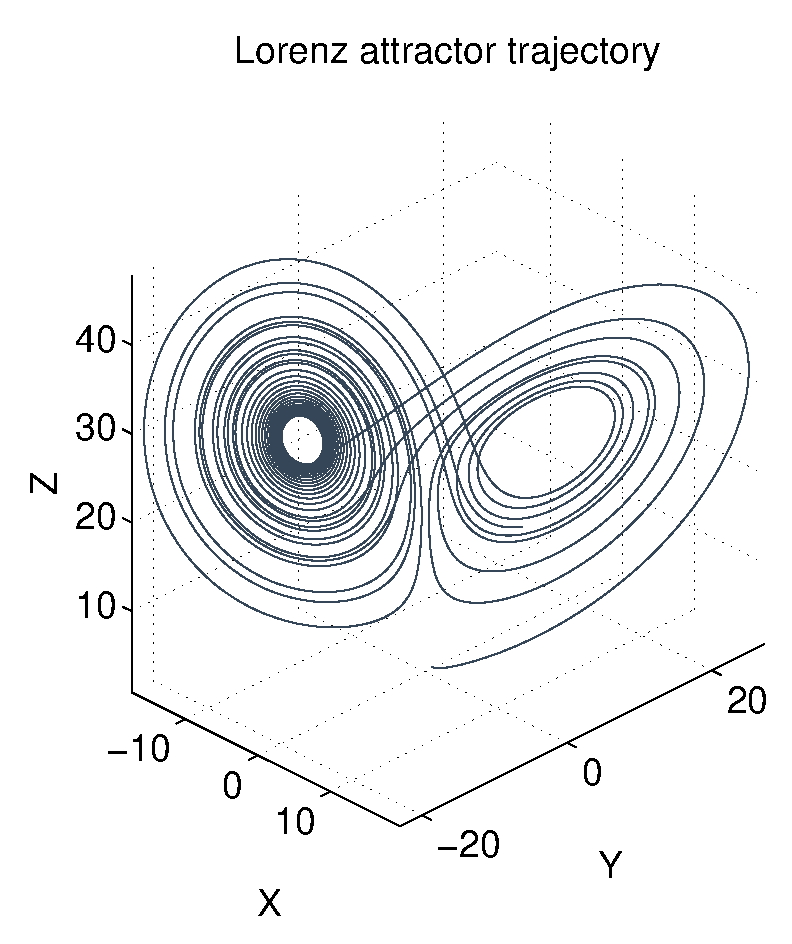
\includegraphics[width=\textwidth]{lorenz}
            \end{figure}
        \end{column}
    \end{columns}
\end{frame}

\note[itemize]{
\item As an example, lets solve a Lorenz attractor system of ordinary
    differential equations.
\item Lorenz attractor is a particle that moves according to these governing
    equations. The plot on the right shows an example of particle trajectory in
    time.
\item We will solve large number of these Lorenz systems at once.  Each of the
    systems will have its own value for parameter R. That's why this is called
    a parameter study.
}

%----------------------------------------------------------------------------
\begin{frame}{Boost.odeint}
    \begin{block}{Общий вид ОДУ}
        \begin{equation*}
            \frac{\mbox{d} x}{\mbox{d} t } = \dot{x} = f(x , t),
            \quad \quad x(0) = x_0.
        \end{equation*}
    \end{block}

    \vspace{\baselineskip}

    \begin{exampleblock}{Применение Boost.odeint:}
        \begin{enumerate}
            \item Определяем тим переменной сосояния (что такое $x$?)
            \item Определяем системную функцию ($f$)
            \item Выбираем алгоритм интегрирования
            \item Выполняем интегрирование по времени
        \end{enumerate}
    \end{exampleblock}
\end{frame}

\note[itemize]{
\item Here is a general form of an ODE.
\item In order to use Boost.odeint, one has to...
}

%----------------------------------------------------------------------------
\begin{frame}[fragile]{Простейшая реализация с VexCL}
    \begin{exampleblock}{1. Тип переменной состояния}
        \begin{lstlisting}
typedef vex::multivector<double, 3> state_type;
        \end{lstlisting}
    \end{exampleblock}

    \begin{exampleblock}{2. Системная функция}
        \begin{lstlisting}[firstnumber=last]
struct lorenz_system {
    const vex::vector<double> &R;

    void operator()(const state_type &x, state_type &dxdt, double t) {
        dxdt = std::tie( sigma * ( x(1) - x(0) ),
                         R * x(0) - x(1) - x(0) * x(2),
                         x(0) * x(1) - b * x(2)  );
    }
};
        \end{lstlisting}
    \end{exampleblock}
\end{frame}

\note[itemize]{
\item We will hold current state of the system (or set of attractor
    coordinates) in a multivector with 3 components.
\item Here is the definition of the Lorenz system functor: It computes the time
    derivative from current state and time (which is not used here).
\item VexCL make the definition of the functor very simple and intuitive: we
    assign a tuple of vector expressions to the multivector that represents
    time derivative.
}

%----------------------------------------------------------------------------
\begin{frame}[fragile]{}
    \begin{exampleblock}{3. Алгоритм (Рунге-Кутты 4-го порядка)}
        \begin{lstlisting}[firstnumber=last]
odeint::runge_kutta4<
        state_type /*state*/,      double /*value*/,
        state_type /*derivative*/, double /*time*/,
        odeint::vector_space_algebra, odeint::default_operations
        > stepper;
        \end{lstlisting}
    \end{exampleblock}
    \begin{exampleblock}{4. Интегрирование}
        \begin{lstlisting}[firstnumber=last]
vex::multivector<double,3> X(ctx, n);
vex::vector<double> R(ctx, n);

X = 10;
R = Rmin + vex::element_index() * ((Rmax - Rmin) / (n - 1));

odeint::integrate_const(stepper, lorenz_system{R}, X, 0.0, t_max, dt);
        \end{lstlisting}
    \end{exampleblock}
\end{frame}

\note[itemize]{
\item Next, we create the stepper object and run the integration routine. Here
    we use classic 4th order Runge-Kutta method.
\item And that's it! This was really easy.
\item And, as you will see from the next slide, it was an order of magnitude
    faster than a multithreaded CPU variant.
}

%----------------------------------------------------------------------------
\begin{frame}[fragile]{Вариант с использованием CUBLAS}
    \begin{itemize}
        \item CUBLAS --- оптимизированная библиотека линейной алгебры от
            NVIDIA.
        \item CUBLAS имеет фиксированный программный интерфейс.
        \item Линейные комбинации (используемые в алгоритмах Boost.odeint):
            \begin{equation*}
                x_0 = \alpha_1 x_1 + \alpha_2 x_2 + \cdots + \alpha_n x_n
            \end{equation*}
            реализованы следующим образом:
    \end{itemize}
    \begin{exampleblock}{}
        \begin{lstlisting}[numbers=none,texcl=true]
cublasDset(...);        // $x_0 = 0$
cublasDaxpy(...);       // $x_0 = x_0 + \alpha_1 * x_1$
...
cublasDaxpy(...);       // $x_0 = x_0 + \alpha_n * x_n$
        \end{lstlisting}
    \end{exampleblock}
\end{frame}

\note{ }

%----------------------------------------------------------------------------
\begin{frame}[fragile]{Вариант с использованием Thrust}
    \begin{itemize}
        \item Библиотека Thrust позволяет получить монолитное ядро:
    \end{itemize}
    \begin{columns}
        \begin{column}{0.70\textwidth}
            \begin{exampleblock}{Thrust}
                \begin{adjustbox}{width=0.95\textwidth,height=0.6\textheight,keepaspectratio}
                    \begin{lstlisting}
struct scale_sum2 {
    const double a1, a2;
    scale_sum2(double a1, double a2) : a1(a1), a2(a2) { }
    template<class Tuple>
    __host__ __device__ void operator()(Tuple t) const {
        thrust::get<0>(t) = a1 * thrust::get<1>(t) + a2 * thrust::get<2>(t);
    }
};

thrust::for_each(
        thrust::make_zip_iterator(
            thrust::make_tuple( x0.begin(), x1.begin(), x2.begin() )
            ),
        thrust::make_zip_iterator(
            thrust::make_tuple( x0.end(), x1.end(), x2.end() )
            ),
        scale_sum2(a1, a2)
        );
                    \end{lstlisting}
                \end{adjustbox}
            \end{exampleblock}
        \end{column}
        \begin{column}<2>{0.22\textwidth}
            \begin{exampleblock}{VexCL}
                \begin{adjustbox}{width=0.95\textwidth,height=0.6\textheight,keepaspectratio}
                    \begin{lstlisting}
x0 = a1 * x1 + a2 * x2;
                    \end{lstlisting}
                \end{adjustbox}
            \end{exampleblock}
        \end{column}
    \end{columns}
\end{frame}

\note{ }

%----------------------------------------------------------------------------
\begin{frame}[fragile]{Производительность (Tesla K40c)}
    \begin{figure}
        \only<1|handout:0> {\includegraphics[width=0.9\textwidth]{perf-1}}%
        \only<2|handout:0> {\includegraphics[width=0.9\textwidth]{perf-2}}%
        \only<3|handout:0> {\includegraphics[width=0.9\textwidth]{perf-3}}%
        \only<4->{\includegraphics[width=0.9\textwidth]{perf-4}}%
    \end{figure}
    \vspace{-1\baselineskip}
    \begin{uncoverenv}<5>
        \begin{itemize}
            \item Недостатки простейшей реализации:
                \begin{itemize}
                    \item Метод Рунге-Кутты использует 4 временных переменных
                        состояния.
                    \item Одна итерация метода приводит к запуску нескольких
                        вычислительных ядер.
                \end{itemize}
        \end{itemize}
    \end{uncoverenv}
\end{frame}

\note{ }

%----------------------------------------------------------------------------
\begin{frame}[fragile]{Специально написанное ядро}
    \begin{columns}
        \begin{column}{0.45\textwidth}
            \begin{itemize}
                \item Создадим монолитное ядро, соответствующее одной итерации
                    Рунге-Кутты.
                \item Будем вызывать это ядро в цикле по времени.
                    \vspace{\baselineskip}
                \item Получим 10-кратное ускорение!
                    \begin{itemize}
                        \item<2|alert@2> \emph{Потеряв универсальность odeint}
                    \end{itemize}
            \end{itemize}
        \end{column} \quad \quad
        \begin{column}{0.5\textwidth}
            \begin{exampleblock}{}
                \begin{adjustbox}{width=0.95\textwidth,height=0.95\textheight,keepaspectratio}
                    \begin{lstlisting}
double3 lorenz_system(double r, double sigma, double b, double3 s) {
    return (double3)( sigma * (s.y - s.x),
                       r * s.x - s.y - s.x * s.z,
                       s.x * s.y - b * s.z);
}
kernel void lorenz_ensemble(
    ulong  n, double dt, double sigma, double b,
    const global double *R,
    global double *X,
    global double *Y,
    global double *Z
    )
{
    for(size_t i = get_global_id(0); i < n; i += get_global_size(0)) {
        double  r = R[i];
        double3 s = (double3)(X[i], Y[i], Z[i]);
        double3 k1, k2, k3, k4;

        k1 = dt * lorenz_system(r, sigma, b, s);
        k2 = dt * lorenz_system(r, sigma, b, s + 0.5 * k1);
        k3 = dt * lorenz_system(r, sigma, b, s + 0.5 * k2);
        k4 = dt * lorenz_system(r, sigma, b, s + k3);

        s += (k1 + 2 * k2 + 2 * k3 + k4) / 6;

        X[i] = s.x; Y[i] = s.y; Z[i] = s.z;
    }
}
                    \end{lstlisting}
                \end{adjustbox}
            \end{exampleblock}
        \end{column}
    \end{columns}
\end{frame}

\note[itemize]{
\item So, what if we did this manually?
\item We would create a single kernel that would do complete Runge-Kutta
    integration step. By the way, here is the kernel that does just that. It's
    very nice-looking kernel in fact.
\item If we run this kernel in a loop, it would give us our solution. And it
    would be ten times faster than our previous variant. So a hundred times
    faster than a CPU! That's an acceleration!
\item But, odeint has 20 different steppers. We don't want to reimplement all
    of those. Let Karsten here do the job, right?
}

%----------------------------------------------------------------------------
\begin{frame}[fragile]{Генерация OpenCL кода из алгоритмов Boost.odeint}
    \begin{itemize}
        \item VexCL определяет тип \code{vex::symbolic<T>}.
        \item Любые операции с переменными этого типа выводятся в текстовый
            поток:
    \end{itemize}
    \begin{exampleblock}{}
        \begin{lstlisting}
vex::symbolic<double> x = 6, y = 7;
x = sin(x * y);
        \end{lstlisting}
    \end{exampleblock}
    \begin{small}
        \begin{verbatim}
double var1 = 6;
double var2 = 7;
var1 = sin( ( var1 * var2 ) );
        \end{verbatim}
    \end{small}
    \pause
    \begin{itemize}
        \item Простая идея:
            \begin{itemize}
                \item Запишем последовательность действий алгоритма.
                \item Сгенерируем монолитное ядро OpenCL.
            \end{itemize}
    \end{itemize}
\end{frame}

\note[itemize]{
\item VexCL allows to achieve same effect without manual coding.
\item The idea is very simple:
    \begin{itemize}
        \item An algorithm (any algorithm) is just a sequence of arithmetic
            expressions.
        \item VexCL symbolic types allow to record such expressions.
    \end{itemize}
}

%----------------------------------------------------------------------------
\begin{frame}[fragile]{Запишем последовательность действий алгоритма
    Boost.odeint}
    \begin{exampleblock}{1. Тип переменной состояния}
        \begin{lstlisting}
typedef vex::symbolic< double >   sym_vector;
typedef std::array<sym_vector, 3> sym_state;
        \end{lstlisting}
    \end{exampleblock}

    \begin{exampleblock}{2. Системная функция}
        \begin{lstlisting}[firstnumber=last]
struct lorenz_system {
    const sym_vector &R;

    void operator()(const sym_state &x, sym_state &dxdt, double t) const {
        dxdt[0] = sigma * (x[1] - x[0]);
        dxdt[1] = R * x[0] - x[1] - x[0] * x[2];
        dxdt[2] = x[0] * x[1] - b * x[2];
    }
};
        \end{lstlisting}
    \end{exampleblock}
\end{frame}

\note[itemize]{
\item Let's record the sequence of expressions that, for example, Runge-Kutta
    method does, and let's build an OpenCL kernel from this sequence.
\item We replace the state type with array of three symbolic variables. We also
    slightly modify our system functor.
}

%----------------------------------------------------------------------------
\begin{frame}[fragile]{}
    \begin{exampleblock}{3. Алгоритм}
        \begin{lstlisting}[firstnumber=last]
odeint::runge_kutta4<
        sym_state /*state*/,      double /*value*/,
        sym_state /*derivative*/, double /*time*/,
        odeint::range_algebra, odeint::default_operations
        > stepper;
        \end{lstlisting}
    \end{exampleblock}

    \begin{exampleblock}{4. Запишем одну итерацию метода Рунге-Кутты}
        \begin{lstlisting}[firstnumber=last]
std::ostringstream lorenz_body;
vex::generator::set_recorder(lorenz_body);

sym_state sym_S = {{ sym_vector(sym_vector::VectorParameter),
                      sym_vector(sym_vector::VectorParameter),
                      sym_vector(sym_vector::VectorParameter) }};
sym_vector sym_R(sym_vector::VectorParameter, sym_vector::Const);

lorenz_system sys{sym_R};
stepper.do_step(std::ref(sys), sym_S, 0, dt);
        \end{lstlisting}
    \end{exampleblock}
\end{frame}

\note[itemize]{
\item We also alter the stepper type accordingly.
\item Next we create the string stream and register it as the expression
    recorder.
\item Finally, we create symbolic variables that would correspond to generated
    kernel parameters, and run single integration step.
\item Now lorenz\_body holds the recorded expression sequence that we
    need.
}

%----------------------------------------------------------------------------
\begin{frame}[fragile]{Сгенерируем монолитное ядро}
    \begin{exampleblock}{5. Сгенерируем и вызовем ядро OpenCL}
        \begin{lstlisting}[firstnumber=last]
auto lorenz_kernel = vex::generator::build_kernel(ctx, "lorenz", lorenz_body.str(),
        sym_S[0], sym_S[1], sym_S[2], sym_R);

vex::vector<double> X(ctx, n), Y(ctx, n), Z(ctx, n), R(ctx, n);

X = Y = Z = 10;
R = Rmin + (Rmax - Rmin) * vex::element_index() / (n - 1);

for(double t = 0; t < t_max; t += dt) lorenz_kernel(X, Y, Z, R);
        \end{lstlisting}
    \end{exampleblock}
\end{frame}

\note[itemize]{
\item We generate the OpenCL kernel named "lorenz" with the information from
    \code{lorenz_body}. We also supply the symbolic vectors that participated
    in our algorithm. Those will become kernel parameters.
\item Next we create our device vectors, and run the integration loop with the
    generated kernel.
\item And this could be done for any of 20 odeint steppers or for almost any
    other generic algorithm!
}

%----------------------------------------------------------------------------
\begin{frame}{Ограничения}
    \begin{itemize}
        \item Строго параллельные алгоритмы (нет взаимодействия между
            потоками).
        \item Не допускаются ветвления в зависимости от текущих значений.
    \end{itemize}
\end{frame}

\note[itemize]{
\item Of course, there are some restrictions.
}

%----------------------------------------------------------------------------
\begin{frame}[fragile]{Производительность сгенерированного ядра}
    \begin{figure}
        \includegraphics[width=\textwidth]{perf-5}
    \end{figure}
\end{frame}

\note[itemize]{
\item But, as you can see from this slide, the technique allows to achieve same
    acceleration we got from manually coded kernel (Both for CPU and GPU).
}

%----------------------------------------------------------------------------
\begin{frame}{Проекты, использующие VexCL}
    \speakerdeck
    \begin{description}[\quad]
        \item[AMGCL] --- решение разреженных СЛАУ алгебраическим многосеточным
            методом:
            \begin{itemize}
                \item \href{https://github.com/ddemidov/amgcl}{github.com/ddemidov/amgcl}
            \end{itemize}
            \vspace{\baselineskip}
        \item[Antioch] --- A New Templated Implementation Of Chemistry for
            Hydrodynamics:
            \begin{itemize}
                \item \href{https://github.com/libantioch/antioch}{github.com/libantioch/antioch}
            \end{itemize}
            \vspace{\baselineskip}
        \item[Boost.odeint] --- численное решение обыкновенных дифуравнений:
            \begin{itemize}
                \item \href{https://github.com/boostorg/odeint}{github.com/boostorg/odeint}
            \end{itemize}
            \vspace{\baselineskip}
        \item[Kratos Multiphysics] --- библиотека численных методов для
            решения\\ прикладных инженерных задач:
            \begin{itemize}
                \item \href{http://www.cimne.com/kratos/}{cimne.com/kratos}
            \end{itemize}
    \end{description}
\end{frame}

\note{ }

\end{document}
